\section{La investigación como parte esencial de la actividad universitaria}

La investigación científica ocupa un papel fundamental en las sociedades actuales. Durante los siglos XX y XXI, los avances científicos han permitido establecer nuestro conocimiento básico del universo y de los fenómenos naturales. Paralelamente, la ciencia ha propiciado el desarrollo tecnológico, transformando profundamente la sociedad y convirtiéndose en un factor de desarrollo económico y humano. Además, en las últimas décadas, se observa cómo el método científico consolida su importancia como una herramienta de pensamiento crítico en el contexto de la era de la información y de la proliferación de contenidos falsos o manipulados.

La universidad ha sido siempre motor y vehículo de la investigación científica. La ley universitaria en su título VII recoge este aspecto de la siguiente forma: ``La investigación científica es fundamento esencial de la docencia y una herramienta primordial para el desarrollo social a través de la transferencia de sus resultados a la sociedad. Como tal, constituye una función esencial de la universidad, que deriva de su papel clave en la generación de conocimiento y de su capacidad de estimular y generar pensamiento crítico, clave de todo proceso científico.'' La función investigadora resulta, por lo tanto, una tarea de carácter central para el profesor universitario e inseparable de su actividad docente. La generación de nuevos conocimientos y el proceso de constante actualización sobre los últimos desarrollos y avances de un campo, repercuten en la calidad de la docencia, que tendrá un carácter vigente y actual. Igualmente, la investigación científica, acerca el método científico a las aulas, fomentando el pensamiento crítico y la elaboración de juicios objetivos. Finalmente, resulta esencial que los resultados científicos deriven en avances que en última instancia proporcionen un retorno positivo a la sociedad.

La Universidad de Cantabria ha mantenido desde sus orígenes un firme compromiso con la investigación científica como prueba el alto nivel de las publicaciones científicas que año tras año salen de sus departamentos e institutos de investigación. En las siguientes líneas, expondré mi plan investigador, centrándome primero en el contexto en el que éste se desarrolla, y describiendo a continuación las principales líneas de investigación que cubrirán tanto aspectos de investigación básica como de investigación aplicada y transferencia de conocimiento. 



\section{Contexto del proyecto investigador}

Este proyecto de investigación se enmarca dentro de la Física Experimental de Altas Energías y de una forma más específica dentro de la Física en Colisionadores. Las dos principales líneas de investigación expuestas en este documento tienen como escenario principal el detector de partículas Solenoide Compacto de Muones (Compact Muon Solenoid, CMS) instalado en el Gran Colisionador de Hadrones (Large Hadron Collider, LHC), así como su evolución tecnológica, que funcionará en el Gran Colisionador de Hadrones de Alta Luminosidad (High Luminosity Large Hadron Collider, HL-LHC) a partir del año 2026. Estas líneas abordarán diferentes aspectos de la Física Experimental de Altas Energías como son el análisis de datos, el desarrollo y optimización de herramientas de reconstrucción y la instrumentación de detectores. La tercera línea de investigación tiene como objetivo la aplicación de algunas de las tecnologías desarrolladas en los detectores de partículas a la resolución de problemas industriales. Finalmente, la última línea tiene que ver con el posicionamiento científico de cara a los nuevos aceleradores que serán construidos en el futuro. Existe además una línea de investigación de carácter transversal que tiene que ver con el desarrollo y aplicación de nuevas técnicas de computación basadas en aprendizaje automático a la resolución de problemas en cada una de las líneas principales. 

\subsection{Física de Altas Energías}


\paragraph{El átomo y el descubrimiento del núcleo\\\\}

La Física de Altas Energías es la disciplina que se encarga del estudio de las componentes fundamentales de la materia y sus interacciones. El origen histórico de esta disciplina se remonta al siglo XVIII, en el momento en el que John Dalton descubre que la materia está compuesta de átomos de diferentes especies, que podían ser clasificados de acuerdo a sus propiedades químicas. En las últimas décadas del siglo XIX, las diferentes especies atómicas habían sido clasificadas en la tabla periódica de los elementos. En esa época, investigaciones de Henri Becquerel y posteriormente de Pierre y Marie Curie y Ernest Rutherford establecieron la existencia de tres tipos diferentes de radiación en la naturaleza (denominadas $\alpha$, $\beta$ y $\gamma$). Paralelamente, J.J. Thomson, en sus investigaciones sobre \emph{rayos catódicos}, descubrió la existencia de los electrones y determinó su masa y su carga, proponiendo un modelo atómico en el que los átomos estaban compuestos por una región de carga positiva que ocupaba la totalidad del volumen del átomo, con algunos electrones de carga negativa insertados en él. En 1911, Rutherford y sus colaboradores desarrollaron una serie de experimentos, consistentes en la interacción de radiación $\alpha$ con una lámina delgada de oro, en los que determinaron que la carga positiva del átomo estaba confinada en una zona minúscula del volumen total del átomo. Rutherford propuso un modelo planetario del átomo en el que los electrones orbitaban un núcleo de carga positiva. En el caso del hidrógeno, el núcleo estaba compuesto por un protón, una partícula con una carga opuesta a la del electrón. Núcleos más pesados estaban compuestos por varios protones.


\paragraph{Teoría cuántica de campos, electrodinámica cuántica y modelo de quarks\\\\}

Durante las primeras décadas del siglo XX, la Mecánica Cuántica y la Teoría de la Relatividad fueron desarrolladas. Bohr, en el año 1913, usó la idea de la cuantización para proponer un model atómico capaz de explicar el espectro de líneas de emisión de los átomos. En la década de 1930, los estudios realizados por Chadwick sobre los núcleos isotópicos, condujeron al descubrimiento del neutrón como una de las componentes del núcleo atómico. Enrico Fermi, a su vez, postuló la existencia de una nueva partícula llamada neutrino, para explicar la aparente no conservación del momento en decaimientos tipo $\beta$ en el núcleo. La sucesiva aplicación de la Mecánica Cuántica a sistemas relativistas, dio lugar a los desarrollos de Paul Dirac para proporcionar una descripción relativista de los electrones que incorporase observables físicos como el spin. Esta descripción predijo también la existencia de la antimateria, que fue confirmada en el año 1932 con el descubrimiento del positrón por parte de Anderson. En esa misma década, el estudio de la radiación cósmica dio lugar al descubrimiento de una nueva partícula llamada muon. En la década de los años cuarenta, Richard Feynman estableció las bases de la electrodinámica cuántica proporcionando una descripción precisa de la interacción entre electrones y fotones. Los desarrollos tecnológicos en los años posteriores dieron lugar a varios experimentos con haces de partículas de alta energía, en los que numerosas partículas inestables fueron descubiertas. Murray Gell-Mann y George Zweig propusieron el modelo de quarks que establecía que la mayor parte de las nuevas partículas eran en realidad estados ligados de unas partículas fundamentales llamadas quarks. 

\paragraph{El Modelo Estándar de las partículas\\\\}

A principios de la década de los setenta, S. Glasgow, S. Weinber y A. Salam propusieron un modelo para las partículas conocido actualmente como el Modelo Estándar  \cite{StandardModel,StandardModel2,StandardModel3,StandardModel4}, en el que la materia está constituida por dos tipos de partículas: leptones y quarks, ambos fermiones, y las fuerzas son transmitidas por el intercambio de bosones: el fotón para la fuerza electromagnética, los bosones W y Z para la fuerza débil y los gluones para la fuerza fuerte. Los leptones y quarks se agrupan en tres familias o \emph{sabores}, de masa creciente. Entre los leptones encontramos al electrón, al muón y al tau y sus respectivos neutrinos, y entre los quarks, los quarks \emph{up} y \emph{down}, \emph{charm} y \emph{strange}, y \emph{top} y \emph{bottom}. Adicionalmente, una nueva partícula, el bosón de Higgs \cite{Higgs, Higgs2, Higgs3, Higgs4, Higgs5, Higgs6, Higgs7} fue predicha como parte de un mecanismo que permitía al resto de partículas adquirir masa. En los años siguientes, la construcción de aceleradores de partículas de potencia creciente, permitieron el descubrimiento del resto de partículas fundamentales del Modelo Estándar: los bosones W \cite{{Wboson}, {Wboson2}} y Z \cite{{Zboson}, {Zboson2}} en el año 1983, el quark top \cite{{TopQuark}, {TopQuark2}} en el año 1995, y finalmente el bosón de Higgs \cite{{HiggsBosonDiscovery}, {HiggsBosonDiscovery2}} en el año 2012.  


\paragraph{Limitaciones del Modelo Estándar\\\\}

A pesar del éxito rotundo del Modelo Estándar describiendo los experimentos realizados hasta la fecha, diferentes argumentos tanto teóricos como experimentales, parecen indicar que se trata de una teoría efectiva a baja energía. 

En primer lugar, desde un punto de vista teórico, el modelo depende de 19 parámetros cuyos valores son determinados experimentalmente pero cuyo origen permanece desconocido. Por otra parte, las correcciones cuánticas recibidas por la masa del bosón de Higgs debido a la presencia de partículas virtuales (fundamentalmente del quark top), deberían conferirle una magnitud comparable a la escala en la que se espera que aparecezca Nueva Física. El hecho de que esto no sea así sugiere la existencia de una increible cancelación o \emph{fine tuning}, que da lugar a lo que comúnmente se refiere como el \emph{problema de la jerarquía}~\cite{{HierarchyProblem}, {HierarchyProblem2}}. El Modelo Estándar sufre también del problema de la \emph{trivialidad cuántica}~\cite{QuantumTriviality} que sugiere la imposibilidad de crear una teoría cuántica de campos consistente, que involucre a un único tipo de bosón de Higgs. Finalmente, el sector \emph{fuerte} del modelo debería incluir un término que permitiese la violación CP (carga y paridad) por parte de la fuerza fuerte. Sin embargo, los experimentos realizados hasta la fecha no han observado jamás dicho tipo de violación~\cite{CPStrong}.

Desde un punto de vista experimental, existen varios fenómenos que el Modelo Estándar no es capaz de explicar. En primer lugar, el modelo no es capaz de incorporar una descripción de la gravedad, quedando esta fuerza al margen del modelo. El modelo tampoco aporta ningún candidato válido para conformar la materia oscura observada en el universo~\cite{DarkMatter}, ni tampoco para explicar el origen de la energía oscura~\cite{DarkEnergy}. Los neutrinos en el Modelo Estándar son partículas no masivas, lo cuál contradice a las medidas de oscilaciones de neutrinos~\cite{Neutrinos} que implican masas distintas de cero para todos los sabores de neutrinos. El mecanismo por el que los neutrinos adquieren masa en el Modelo Estándar no está completamente bien establecido. Por último, el Modelo Estándar no es capaz de explicar la asimetría observada en el universo entre la materia y la antimateria.

\paragraph{Física más allá del Modelo Estándar (Nueva Física)\\\\}

En las últimas décadas, varias extensiones al Modelo Estándar han surgido para intentar resolver total o parcialmente los problemas mencionados. La Supersimetría (SUSY)~\cite{SuperSymmetry}, es una de las que ha gozado de mayor popularidad en los últimos años. Este modelo postula la existencia de una simetría universal que asigna un bosón (fermión) a cada fermión (bosón) del Modelo Estándar. Las partículas supersimétricas de los fermiones contribuyen a la cancelación de las correcciones radiativas a la masa del bosón de Higgs, resolviendo así el problema de la jerarquía. A su vez, combinaciones lineales de las partículas supersimétricas de los bosones del Modelo Estándar, dan lugar a partículas masivas y neutras que resultan candidatas idóneas para conformar la materia oscura. Otros modelos, conocidos comúnmente como \emph{modelos con dimensiones extra}~\cite{{ExtraDimensions}, {ExtraDimensions2}, {ExtraDimensions3}}, postulan la existencia de dimensiones espacio-temporales adicionales en las que sólo la gravedad puede operar. Estos modelos, por tanto, son capaces de proporcionar una descripción para la fuerza gravitatoria y de resolver a la vez el problema de la jerarquía. Muchos de estos ingredientes (SUSY, dimensiones extra) son recogidos en la \emph{teoría de cuerdas}~\cite{StringTheory} en la que se abondona la concepción puntual de las partículas para dotarlas de un grado de libertad adicional en forma de longitud (cuerda). Este tipo de teoría es referida con frecuencia como \emph{teoría del todo} por su capacidad para describir la gravedad y para proporcionar la \emph{Gran Unificación} de las Fuerzas~\cite{GUT} en escalas altas de energía. Otras extensiones populares del Modelo Estándar incluyen los modelos de \emph{Higgs compuesto}~\cite{Composite}, en los que el bosón de Higgs se postula como un estado ligado de algún tipo nuevo de interacción fuerte.

Todos estos modelos de Nueva Física y otros no mencionados, predicen la existencia de nuevas partículas desconocidas hasta la fecha. Dichas partículas pueden ser detectadas en experimentos de colisión tanto de forma indirecta, a través de medidas de precisión de procesos del Modelo Estándar, para determinar posibles desviaciones provocadas por las correcciones cuánticas inducidas por las nuevas partículas; como de forma directa, produciéndolas en su forma resonante y determinando su presencia a través de sus productos de desintegración.   


\subsection{El Gran Colisionador de Hadrones}

El LHC~\cite{LHC} es un colisionador de protones circular con una longitud de 27~km. Se encuentra alojado 100~metros bajo tierra atravesando la frontera franco-suiza en las proximidades de la ciudad de Ginebra. El acelerador se encuentra formado por un total de 8 sectores circulares de 2460~m, conectados por 4 regiones rectas de 540~m en los que los experimentos están ubicados. El acelerador está compuesto por 1232 imanes de tipo dipolo con cavidades de radiofrecuencia con capacidad para incrementar la energía de los protones 0.5~MeV en cada vuelta. El LHC acelera dos haces de protones en direcciones opuestas, haciendo que colisionen en 4 puntos alrededor de los cuales se han construido cuatro experimentos: ALICE~\cite{ALICEDetectorPaper}, ATLAS~\cite{ATLASDetectorPaper}, CMS~\cite{CMSDetectorPaper} y LHC-b~\cite{LHCbDetectorPaper}. Una vista esquemática del acelerador puede verse en la figura \ref{fig:lhc}. El número de sucesos de un proceso específico, producidos por unidad de tiempo en un acelerador viene dado por la probabilidad específica de dicho proceso (dada como una sección eficaz) y una magnitud conocida como luminosidad instantánea. La energía de diseño del LHC para cada haz de protones es de 7 TeV y su luminosidad instantánea nominal es L=10$^{34}$~cm$^{-2}$~s$^{-1}$, dando lugar a alrededor de 10$^{10}$ interacciones protón-protón por segundo.       

\begin{figure}[ht]
\centering
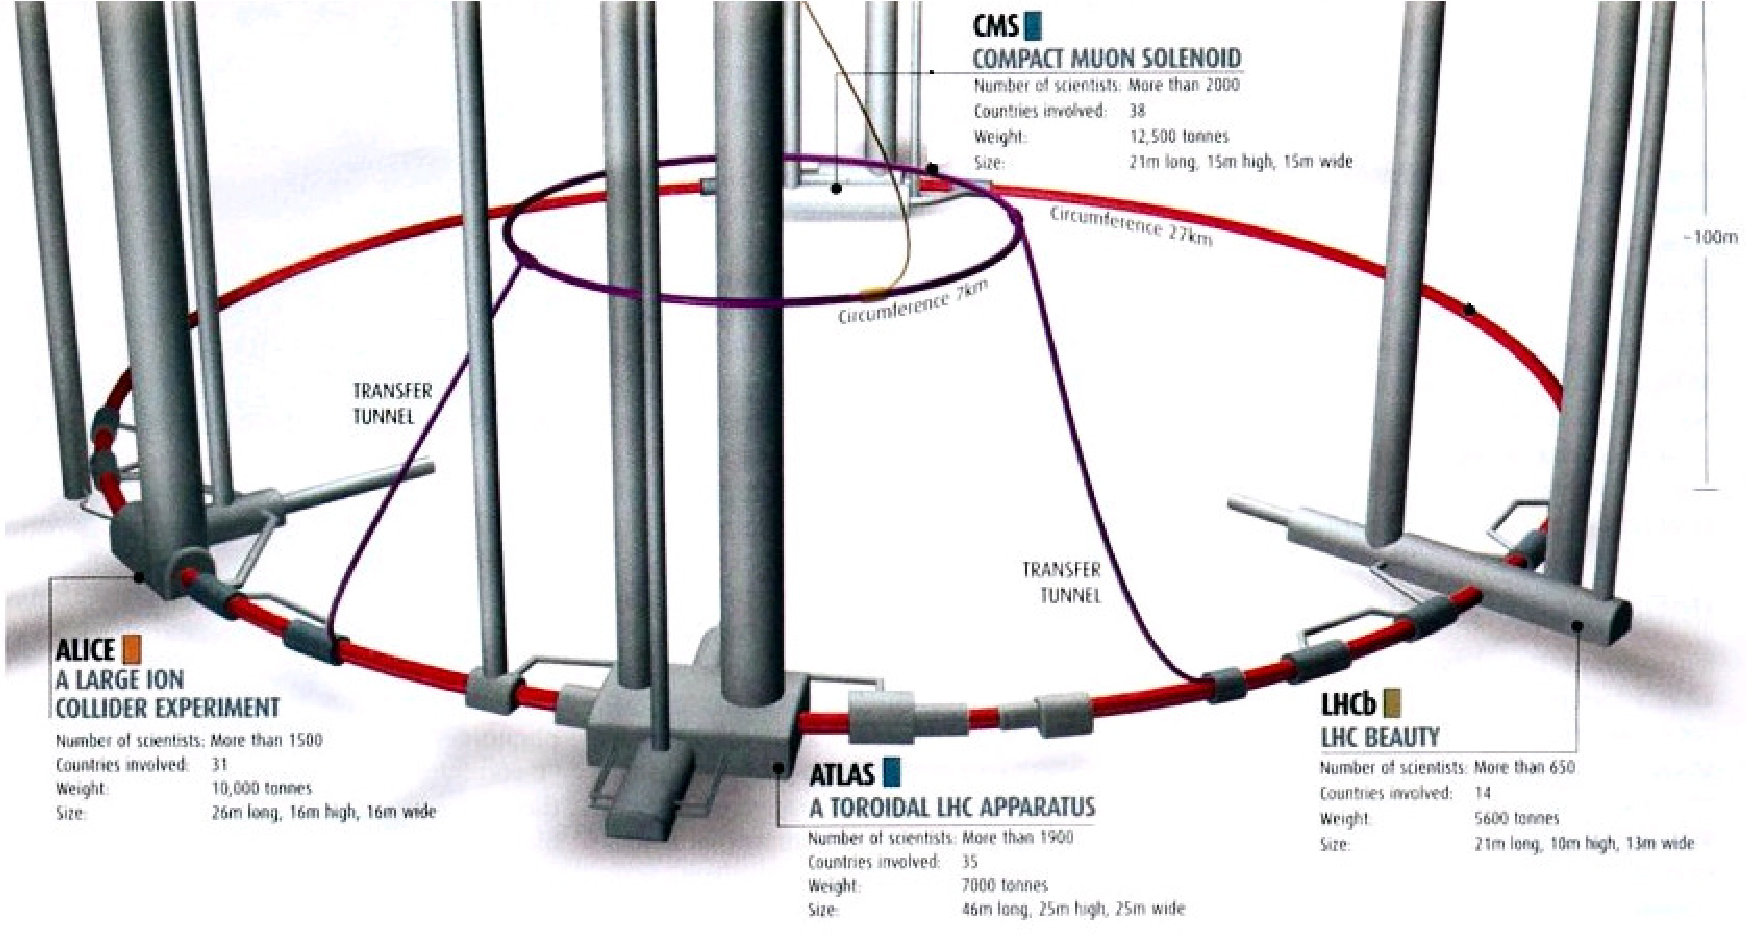
\includegraphics[height=5.3cm]{fig/accelerator-view.pdf}
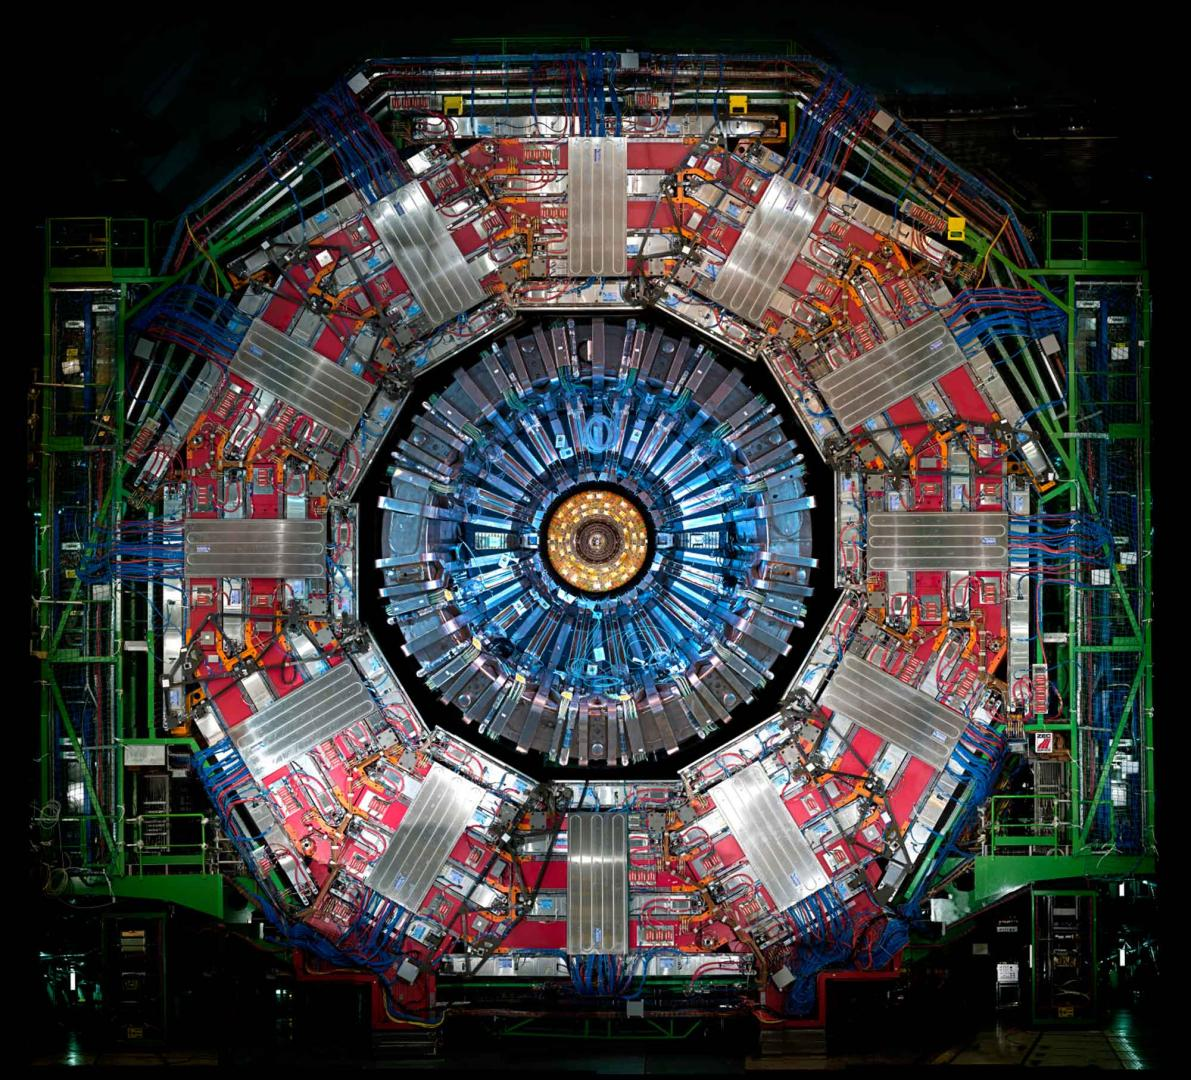
\includegraphics[height=5.3cm]{fig/cms-detector-cern.jpg}
\caption{Esquema del LHC incluyendo la localización de los cuatro experimentos, así como parte de la cadena de aceleración e inyección (izquierda). Fotografía transversal del detector CMS (derecha).}
\label{fig:lhc}
\end{figure} 

El LHC comenzó su funcionamiento en el año 2010 operando durante los años 2010-2012 a una energía del centro de masas de $\sqrt{s}$=7-8~TeV. En este periodo, conocido como Run 1, se acumuló una luminosidad integrada de aproximadamente 30~fb$^{-1}$. Durante los años 2013 y 2014, el LHC permaneció inactivo para realizar actividades de mantenimiento y mejora. En el año 2015, comenzó el llamado Run 2, con una energía del centro de masas de $\sqrt{s}$=13~TeV. Durante la duración total del Run 2, comprendiendo los años 2016, 2017 y 2018 el LHC acumuló una luminosidad integrada de aproximadamente 150~fb$^{-1}$. En el año 2022, se espera que el LHC comience el Run 3, con una energía del centro de masas aún por determinar, en el rango $\sqrt{s}$=13-14~TeV y con una previsión de luminosidad integrada de otros 150~fb$^{-1}$ aproximadamente. 


\subsection{El Solenoide Compacto de Muones}

El Solenoide Compacto de Muones, CMS, es un detector de propósito general instalado en el P5 (punto 5) del LHC, en la proximidad del pueblo de Cessy en Francia. Las componentes principales de CMS son: el sistema de \emph{tracking}, basado completamente en tecnología de silicio;  el calorímetro electromagnético formado por cristales centelleadores; el calorímetro hadrónico, con estructura de sandwhich en capas de latón y centelleador; el imán superconductor capaz de proporcionar un campo de 3.8~T en la zona central del detector; y finalmente el sistema de muones, con cámaras que utilizan tecnología de tubos de deriva, de tiras catódicas y de placas resistivas. La figura~\ref{fig:lhc} (derecha) muestra una fotografía del detector CMS en su vista transversal. El detector está dotado además de un sistema de disparo o \emph{trigger} con dos niveles, uno basado en hardware y conocido como trigger de nivel 1 (L1) y otro basado en software y conocido como trigger de alto nivel (HLT). Ambos sistemas conjuntamente seleccionan los sucesos más interesantes desde un punto de vista físico, efectuando una reducción de 7-8 órdenes de magnitud y proporcionando una tasa final de 1000 sucesos por segundo. Estos sucesos son almacenados y posteriormente procesados utilizando la estructura de computación de CMS, basada en el concepto GRID y con centros de computación distribuidos por todo el mundo. 

Las prestaciones más importantes del detector CMS incluyen una excelente identificación de muones y resolución de momento sobre un amplio rango de momento y pseudorapidez; buena resolución del momento de partículas cargadas y alta eficiencia de reconstrucción en el \emph{tracker}; buena resolución de energía en el calorímetro electromagnético, con buena resolución en la masa invariante de pares de fotones y electrones; y buena resolución de la energía en el calorímetro hadrónico, incluyendo buena resolución en la masa invariante de parejas de jets y con una alta hermeticidad (hasta 5 en pseudorapidez).


\subsection{El programa de física del LHC}

El LHC permite realizar estudios detallados de un amplio rango de aspectos del Modelo Estándar, así como de búsquedas de física más allá de él. Uno de los objetivos principales del LHC consiste en el estudio del mecanismo de ruptura de simetría electrodébil, primero con la detección del bosón de Higgs, que tuvo lugar en el año 2012, y luego con la medida detallada de sus propiedades. La búsqueda de física más allá del modelo estándar, constituye otro de los ejes principales del programa de física del acelerador. En términos muy generales, se puede condensar el programa de física del LHC en los siguientes elementos:

\begin{itemize}
    \item Estudio del mecanismo de ruptura de simetría, el bosón de Higgs y sus propiedades.
    \item Búsquedas de Nueva Física: Supersimetría, dimensiones extra, etc.
    \item Estudios de Quantum Electrodynamics (QCD) y física con multi-jets.
    \item Estudio de la física del quark top.
    \item Medidas de la Matriz CKM a través de estudios de violación CP en el sector de Bs.
    \item Estudio de propiedades del plasma de quark-gluones en colisiones de iones pesados.
\end{itemize}

Los datos recogidos por CMS y ATLAS durante el Run 1 y 2, han permitido profundizar en varios aspectos de este programa. El elemento más relevante es sin duda el descubrimiento del bosón de Higgs en el año 2012, usando la combinación de los canales de desintegración $H\rightarrow\gamma\gamma$, $H\rightarrow W^{+}W^{-}$, $H\rightarrow ZZ$, $H\rightarrow b\bar{b}$ y $H\rightarrow\tau\tau$. En los meses y años posteriores, se estimaron las propiedades del nuevo bosón tales como la masa~\cite{Hmass1,Hmass2}, las fracciones de desintegración~\cite{Hcoup1,Hcoup2} o el espín\cite{Hspin1,Hspin2}. También se produjeron estudios atendiendo a los modos de producción del bosón de Higgs (fusión de gluones y fusión de bosones vector) y se observaron desintegraciones de sección eficaz más pequeña como la desintegración $H\rightarrow\tau\tau$~\cite{Htautau1,Htautau2}, y $H\rightarrow\mu\mu$\cite{Hmumu1,Hmumu2}. En los últimos años también se han observado procesos de producción del bosón de Higgs en asociación con pares de quarks top-antitop ($t\bar{t}H$)~\cite{tth1,tth2}. 

La física del quark top ha sido estudiada con gran nivel de detalle durante los primeros años de funcionamiento del LHC. Medidas de la sección eficaz total y diferencial de la producción de pares de quarks top-antitop en sus diferentes canales de desintegración~\cite{topcross1,topcross2,topcross3,topcross4}, así como de la producción de \emph{single-top}~\cite{singletop1,singletop2} han sido realizadas con algo grado de precisión. Otras propiedades, como su masa~\cite{topmass1,topmass2}, han sido también estudiadas de forma exhaustiva.

\begin{figure}[ht]
\centering
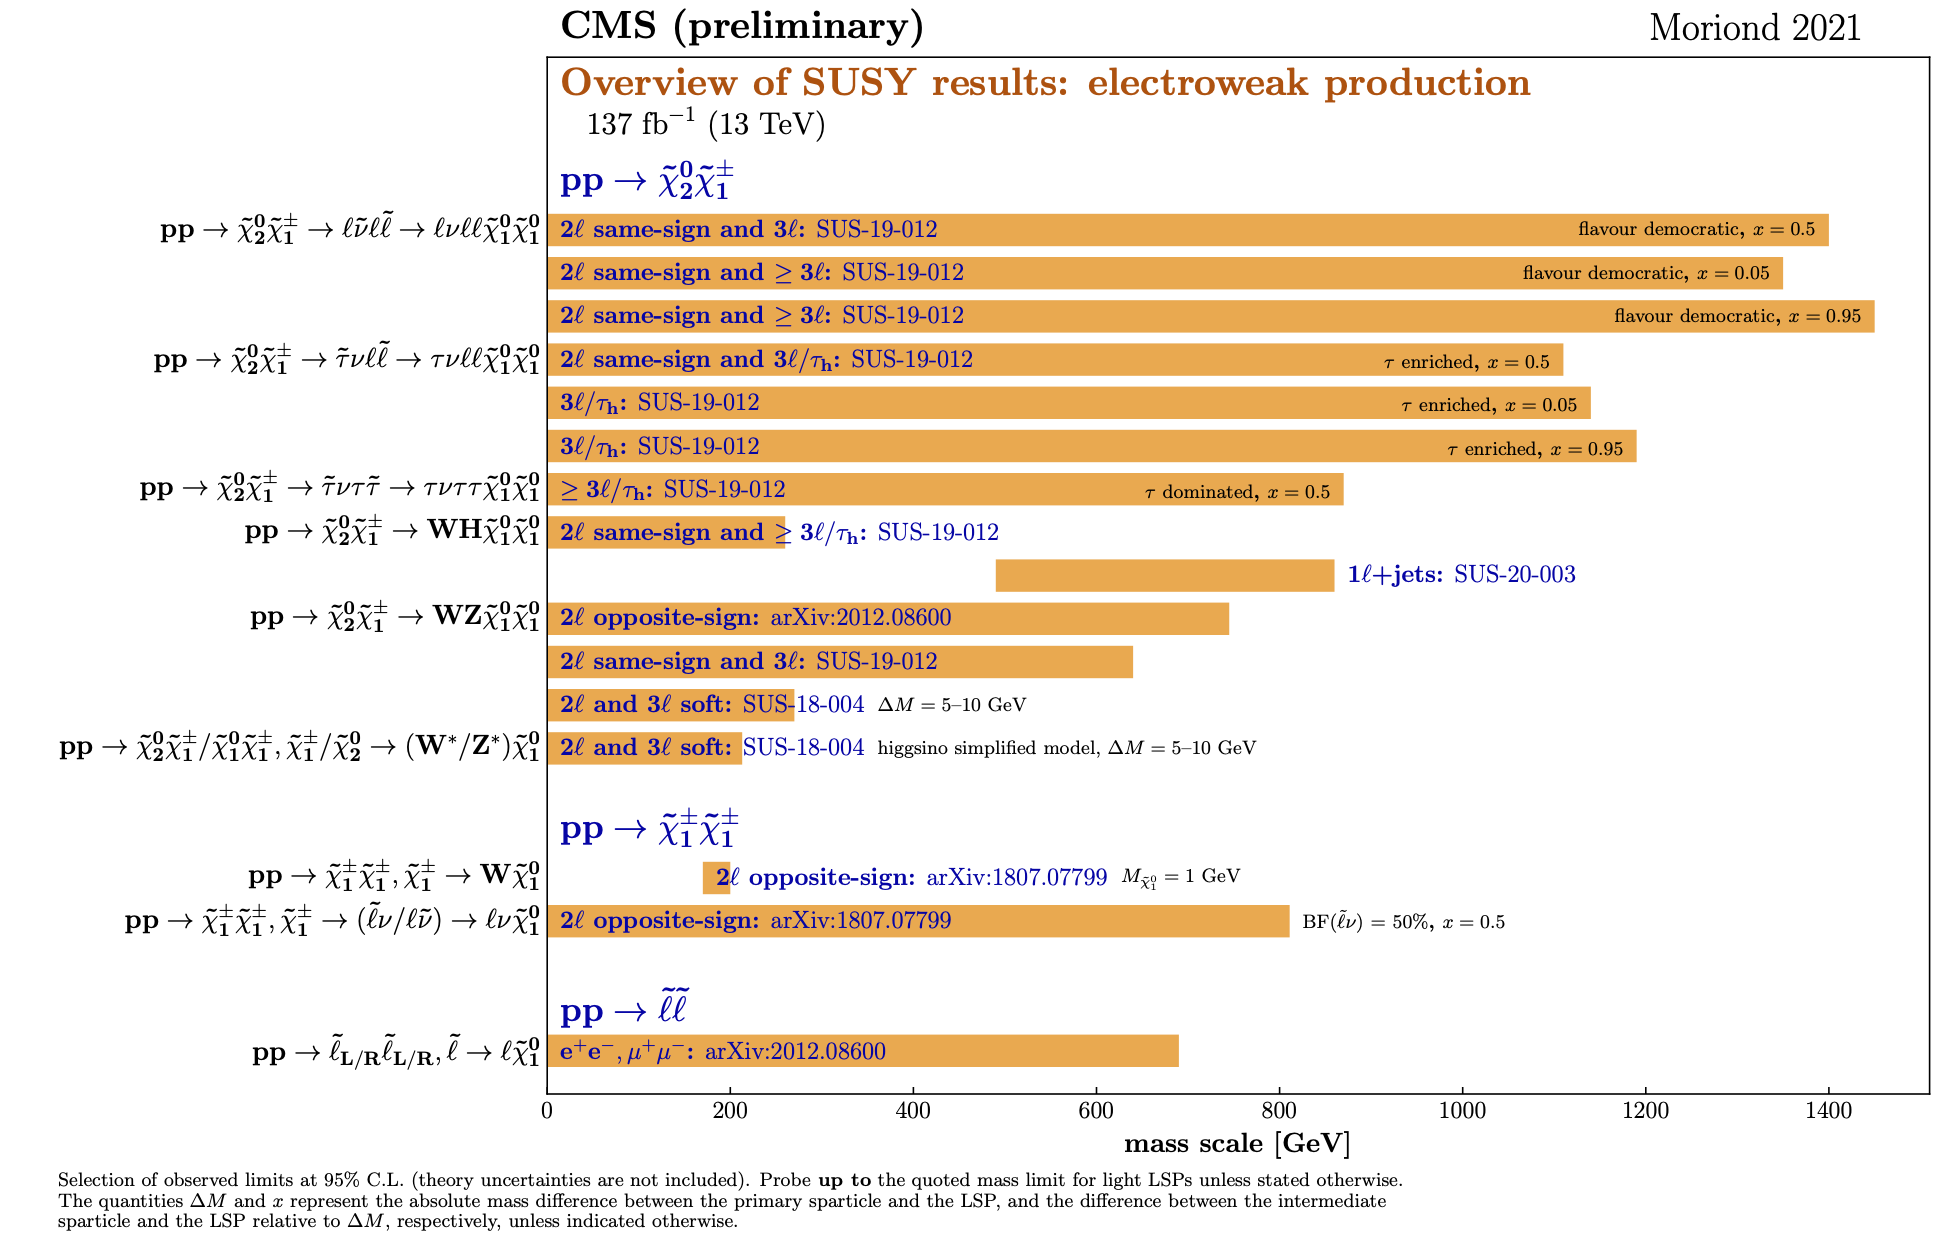
\includegraphics[height=5.0cm]{fig/barplot_EWK.png}
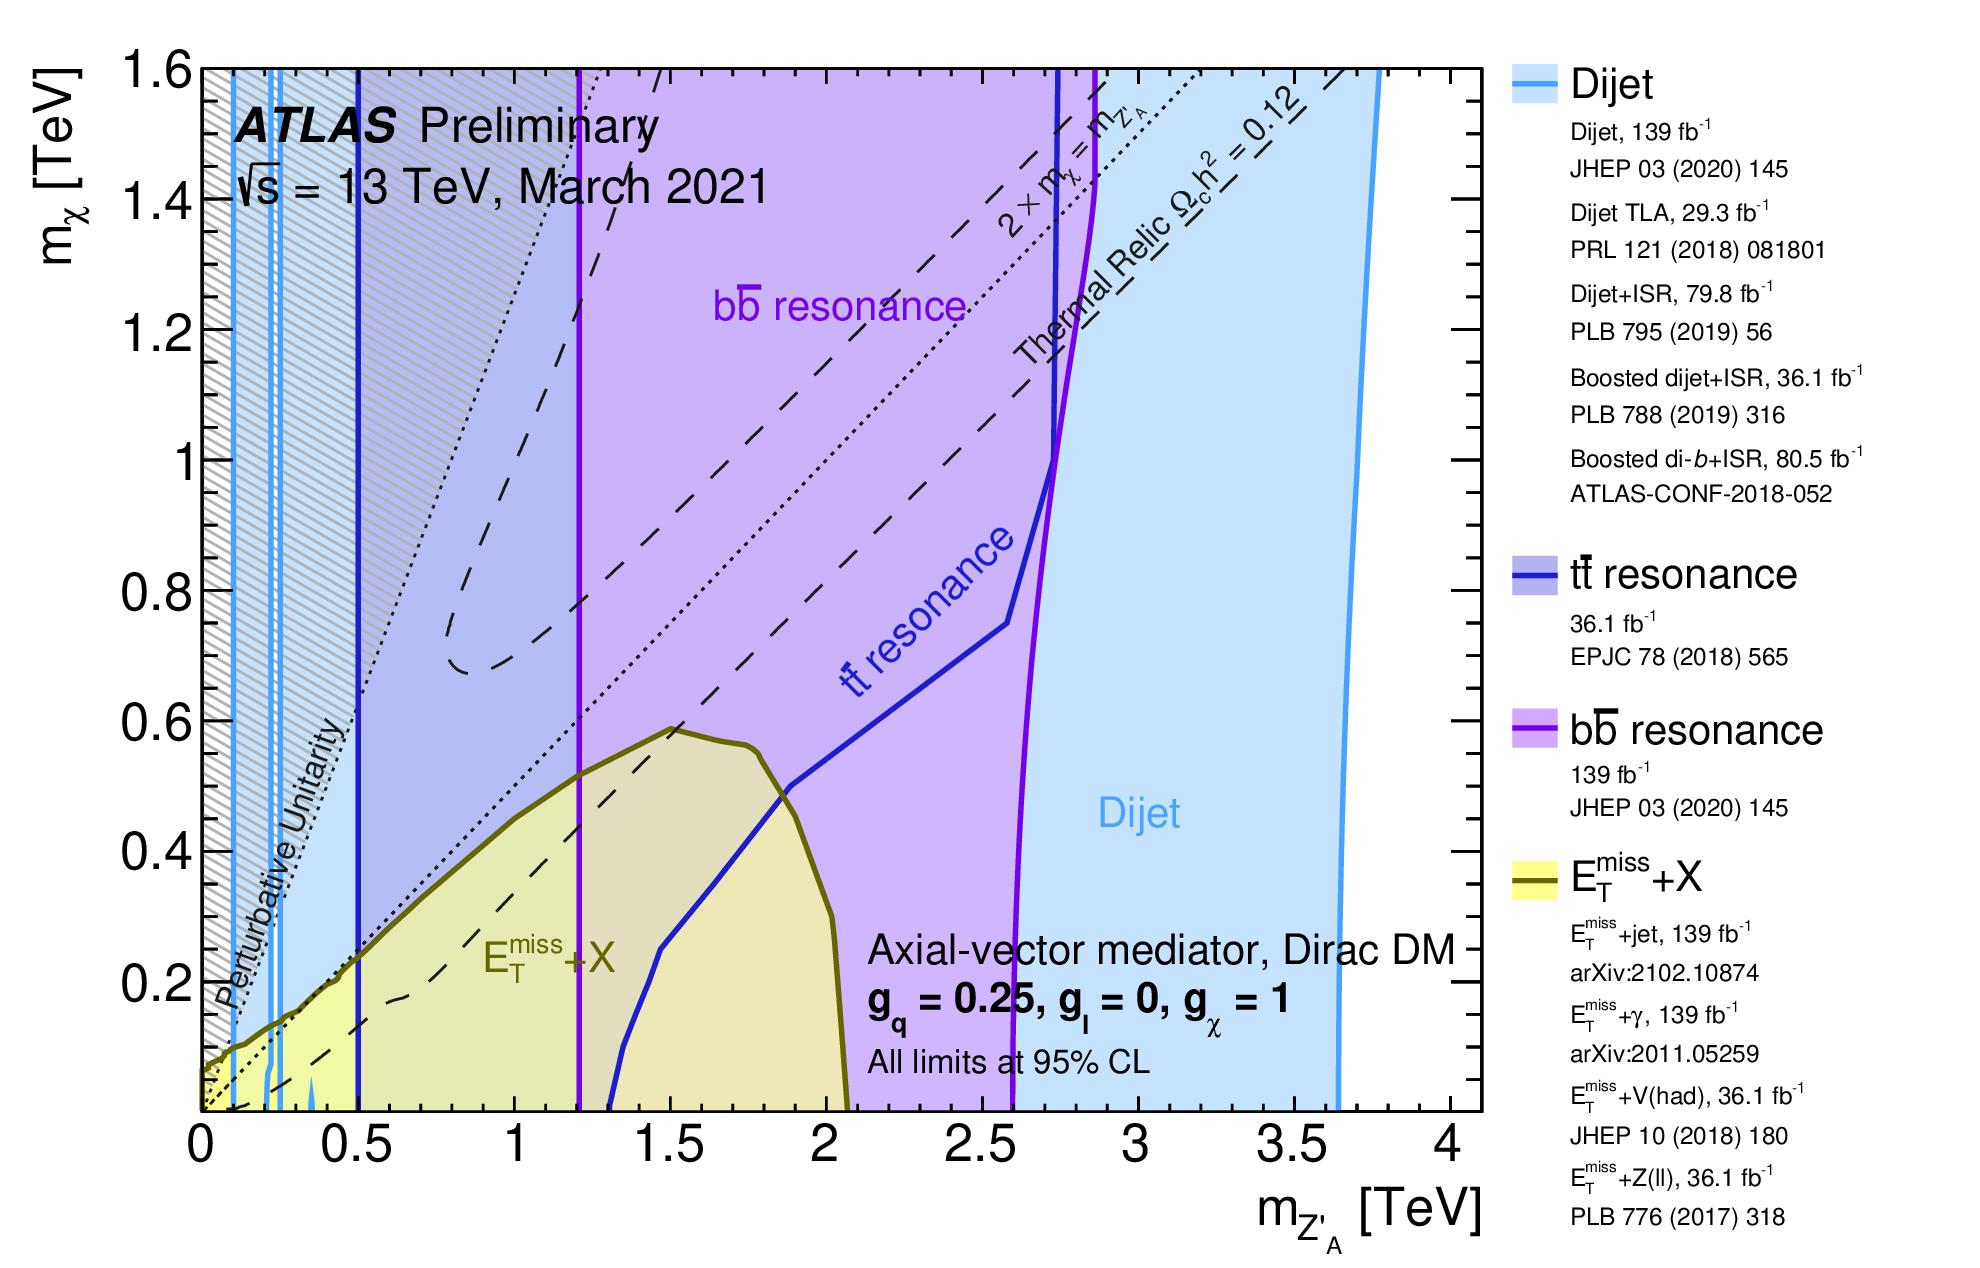
\includegraphics[height=5.0cm]{fig/fig_01.png}
\caption{Resumen de exclusiones en las masas de partículas supersimétricas producidas de forma electrodébil (izquierda). Zonas de exclusión en el plano de masa de la partícula de materia oscura y masa del mediador para el caso de mediadores leptofóbicos de tipo axial-vector (derecha).} 
\label{fig:newphysics}
\end{figure} 

Pese al éxito rotundo del LHC y de sus experimentos, durante el Run 1 y 2, ningún indicio de nueva física ha sido observado. Tanto CMS como ATLAS han contado con ambiciosos programas de búsqueda de Nueva Física, en los que se han realizado búsquedas inspiradas en modelos supersimétricos, modelos con dimensiones extra, búsquedas de materia oscura o búsquedas de resonancias de alta masa, entre otros. El espacio de parámetros de dichos modelos ha sido constreñido a través del establecimiento de límites superiores a su sección eficaz de producción. Además de las búsquedas directas, búsquedas indirectas de nueva física, como la medida de la sección eficaz de la desintegración del bosón $B_s\rightarrow\mu\mu$~\cite{bsmumu2,bsmumu1} producida en LHC-b y CMS, parecen dificultar la existencia de una Nueva Física fácilmente accesible. De la misma forma, la masa del Bosón de Higgs, m$_H=$~125~GeV, impone fuertes restricciones a las teorías supersimétricas, que para resolver el problema de la jerarquía han de permitir grandes correcciones de squarks stop, o una gran fracción de \emph{mixing} entre ellos. Las figuras~\ref{fig:newphysics} muestran algunas de las exclusiones realizadas hasta la fecha en las masas de diferentes partículas supersimétricas (izquierda) y en el contexto de modelos de materia oscura (derecha). 

La aparente ausencia de indicios de Nueva Física ha dada lugar a un aumento del interés por búsquedas en topologías no tradicionales como son las búsquedas de partículas con larga vida media, \emph{Heavy Stable Charge Particles}, topologías con trazas \emph{desvanecientes}, etc. Los algoritmos de reconstrucción de los experimentos no están optimizados para este tipo de objetos, siendo posible que de manifestarse la Nueva Física en este tipo de topologías, los experimentos fallasen en encontrarla. Este argumento justifica el creciente interés por este tipo de búsquedas y también por el desarrollo de algoritmos que permiten captar este tipo de topologías. 

\subsection{El High Luminosity Large Hadron Collider}

\paragraph{El HL-LHC\\\\}

El High-Luminosity Large Hadron Collider (HL-LHC)~\cite{HLLHC} será instalado en el túnel ocupado actualmente por el LHC y comenzará a funcionar en el año 2027. Este acelerador aumentará en un orden de magnitud la luminosidad integrada que recogerá el LHC desde los 300~fb$^{-1}$ hasta los 3000~fb$^{-1}$. Este objetivo ha requerido un gran salto tecnológico que incluye la fabricación de nuevos y más poderosos imanes de enfocado (12~T, en lugar de los 8~T del LHC) y de curvatura (11~T, en lugar de 8.3~T en el LHC); nuevas líneas de transmisión superconductoras con capacidad para conducir intensidades de hasta 100000 A; o la renovación de la cadena de aceleración, entre otros aspectos.

El programa de física del HL-LHC extiende el del LHC persiguiendo realizar medidas mucho más precisas de las propiedades del bosón de Higgs y de sus \emph{couplings} (como por ejemplo del \emph{trilinear coupling} a través de la medida del proceso de producción de pares de Higgs); estudios de QCD como la medida de las \emph{parton distribution functions} (pdfs), o análisis de sucesos con alto \emph{q$^2$}; o búsquedas de Nueva Física, con énfasis en resonancias de alta masa, partículas de larga vida media o búsquedas de Materia Oscura. 

\paragraph{El ``Phase-2 Upgrade'' de CMS\\\\}

El HL-LHC impondrá nuevas y exigentes condiciones de operación a los experimentos. La alta luminosidad instantánea del nuevo acelerador requerirá que los experimentos desarrollen nuevos y más rápidos sistemas de trigger; por otro lado el aumento en el número de colisiones espúreas (pile-up) incrementará sustancialmente la ocupancia en los detectores y la multiplicidad de trazas. Con objeto de adaptarse a estas nuevas condiciones, los experimentos se encuentran en proceso de mejora y renovación de sus sistemas. 

La colaboración CMS se encuentra actualmente en proceso de diseño y construcción de sus nuevos sistemas. Concretamente, CMS instalará un nuevo \emph{tracker} de silicio~\cite{upgradeTracker} con un mayor número de canales y una resolución espacial mejorada. El detector de píxeles será también mejorado y extendido para cubrir un mayor rango de pseudorapidez. Además, el uso de nuevas tecnologías de computación, como las FPGA, permitirá la mejora de los sistemas de trigger para que sean capaces de utilizar la información del tracker a nivel L1~\cite{upgradeL1}. Los calorímetros serán otro elemento innovador, usando una nueva tecnología que permitirá disponer de una mayor granularidad y de la capacidad de realizar medidas tridimensionales de los depósitos de energía de las partículas incidentes~\cite{upgradeBarrel, upgradeEndcap}. El sistema de muones y otros sub-sistemas serán también transformados o extendidos~\cite{upgradeMuon}. Además, CMS será dotado de un detector completamente nuevo: \emph{el MIPs Timing Detector (MTD)}.

\paragraph{El MIPs Timing Detector\\\\}

El MTD~\cite{MTDTDR} es un nuevo detector con capacidad para medir el tiempo de paso de las partículas cargadas con una precisión de unos 40~ps al principio de operación y unos 60~ps al final de su vida útil. Este detector está compuesto por una zona \emph{Barrel}, \emph{Barrel Timing Layer (BTL)} y dos \emph{Endcaps}, \emph{Endcap Timing Layer (ETL)}, que serán instalados a continuación del tracker, dentro del tubo de soporte de su barril, y en la nariz del calorímetro, respectivamente. La Fig.~\ref{fig:mtd} muestra un diagrama del MTD con sus componentes. La tecnología de detección usada en el BTL estará basada en cristales centelleadores (cristales de LYSO), mientras que el ETL utilizará tecnología basada en sensores de silicio y más concretamente de sensores LGAD \emph{Low Gain Avalanche Diodes}~\cite{LGAD1,LGAD2}.


\begin{figure}[ht]
\centering
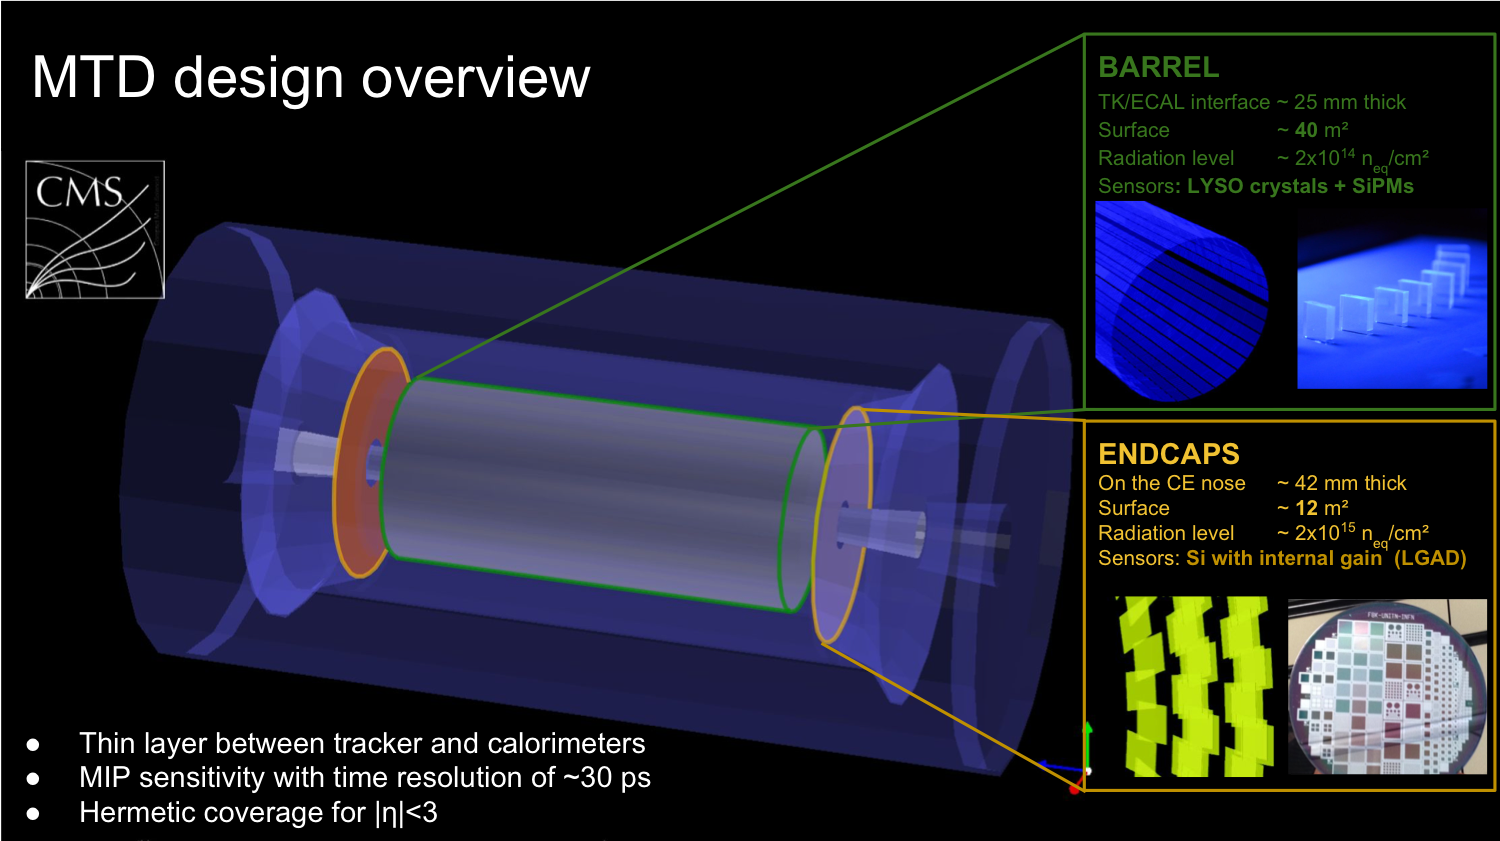
\includegraphics[width=10cm]{fig/Timing_schematic_fancy.png}
\caption{Esquema del MIPs Timing Detector con la zona del barril, BTL, con tecnología de cristales centelleadores (LYSO) y la zona \emph{endcap}, ETL, con tecnología de LGADs.}
\label{fig:mtd}
\end{figure} 

El MTD tendrá un papel fundamental en el contexto del HL-LHC como un instrumento para reducir los altos niveles de pile-up que producirá dicho acelerador. La asignación del tiempo de producción a cada traza, permitirá añadir una nueva coordenada a la discriminación de trazas y vértices, reduciendo de esta forma los niveles de pile-up, desde los 200 esperados en el HL-LHC hasta niveles parecidos al actual LHC. El MTD, además, abrirá posibilidades únicas en muchos sectores del programa de física de CMS, como por ejemplo, en las búsquedas de partículas de larga vida media, ya que permitirá medir además de su desplazamiento, su retraso temporal. El MTD también permitirá realizar una identificación de partículas basándose en su tiempo de vuelo \emph{Time-Of-Flight Id}, lo cuál tendrá importantes repercusiones en varios análisis y muy especialmente en la física de iones pesados. 



\section{Análisis de datos con el experimento CMS}

Esta línea de investigación persigue la búsqueda de evidencias de Nueva Física en los datos recogidos por el experimento CMS tanto durante el Run 3 del LHC como durante la operación del HL-LHC. Varios modelos de Nueva Física serán estudiados incluyendo modelos supersimétricos, modelos exóticos con presencia de Materia Oscura, y modelos exóticos con partículas de larga vida media. También se prestará atención al proceso de producción de \emph{pares de Higgs} para estudiar posibles desviaciones con respecto al Modelo Estándar. El factor común a todos los análisis será la presencia de al menos un leptón (electrón o muon) en los estados finales de los modelos de señal. En el desarrollo de esta línea de investigación adquirirá también un papel fundamental el uso de técnicas modernas de computación basadas en aprendizaje automático como herramienta para optimizar el alcance de los diferentes análisis. El objetivo de esta línea de investigación es el posible descubrimiento de nuevas partículas, o en su defecto, el establecimiento de límites estadísticos a sus secciones eficaces de producción, para constreñir el espacio de parámetros de los modelos estudiados.

\subsection{Experiencia previa}

\paragraph{Búsquedas de SUSY con leptones del mismo sabor y carga opuesta\\\\}

Mi experiencia en búsquedas de Nueva Física en el experimento CMS comienza en el año 2010 con mi incorporación al \emph{Swiss Federal Institute of Technology Zürich} (ETHZ) como investigador postdoctoral y ha continuado de forma ininterrumpida hasta la actualidad. Durante los años 2010 a 2017 mi actividad investigadora estuvo centrada en las búsquedas de Supersimetría. Concretamente, durante este periodo me convertí en referente y líder, dentro de la colaboración CMS, de uno de los análisis principales del grupo de SUSY: las búsquedas en sucesos con dos leptones del mismo sabor y carga opuesta. En este contexto, lideré durante años a un grupo de doctorandos y postdocs de varias universidades, y supervisé a dos doctorandos dentro de la ETHZ en esta temática. Mi contribución a esta saga de análisis, que dio lugar a 8 publicaciones~\cite{{Edge1},{Edge2},{Edge3},{Edge4},{Edge5},{Edge6},{Edge7},{Edge8}}, fue integral, pasando por el diseño global del análisis y las herramientas de software, hasta el diseño de los métodos de predicción de fondo, el análisis estadístico y las funciones de \emph{persona de contacto} de cara a la colaboración CMS. Resulta relevante mencionar, que uno de estos análisis, el realizado con los datos recogidos con $\sqrt{s}=$8~TeV presentó un exceso de datos en la masa invariante de los leptones con una significancia de 2.9~ $\sigma$ (ver~ Fig.\ref{fig:edge}). El análisis fue sometido a un proceso de escrutinio sin precedentes por parte de la colaboración y debido a ello fue reconocido como el análisis más robusto hasta la fecha. Este exceso supuso también el mayor indicio de Nueva Física hasta la fecha en CMS, atrayendo la atención de la comunidad de teóricos. Como resultado de estos trabajos la colaboración CMS me seleccionó para presentar estos resultados de CMS en conferencias tan importantes como las ediciones de ICHEP (International Conference in High Energy Physics) en 2012 y en 2014. Por otro lado, además de este tipo de análisis, también tuve contribuciones a otras búsquedas de Supersimetría como son las búsquedas con leptones de la misma carga~\cite{SameSign, SameSign2, SameSign3, SameSign4}, o las búsquedas hadrónicas utilizando la variable MT2~\cite{MT2, MT22, MT23, MT24}. 


\begin{figure}[ht]
\centering
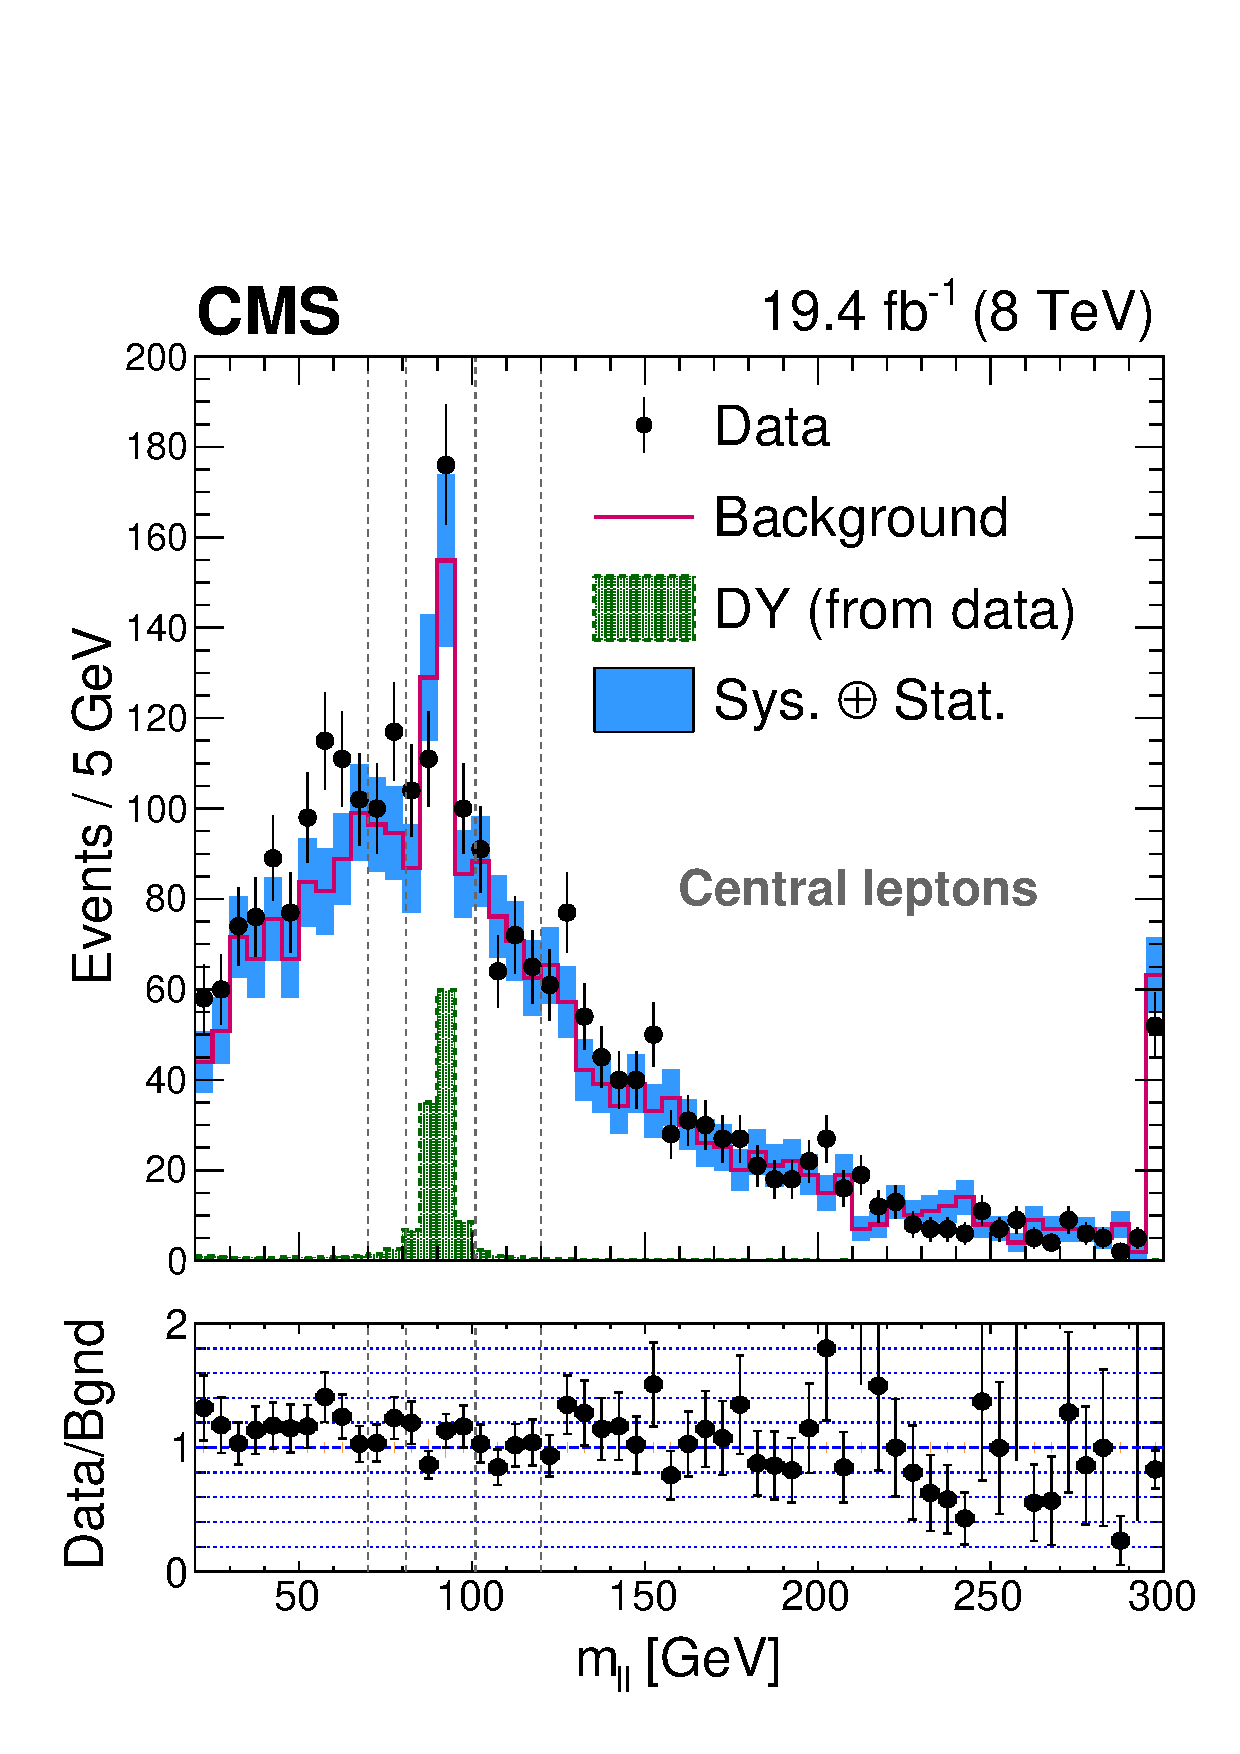
\includegraphics[height=7.3cm]{fig/CNC_CE.pdf}
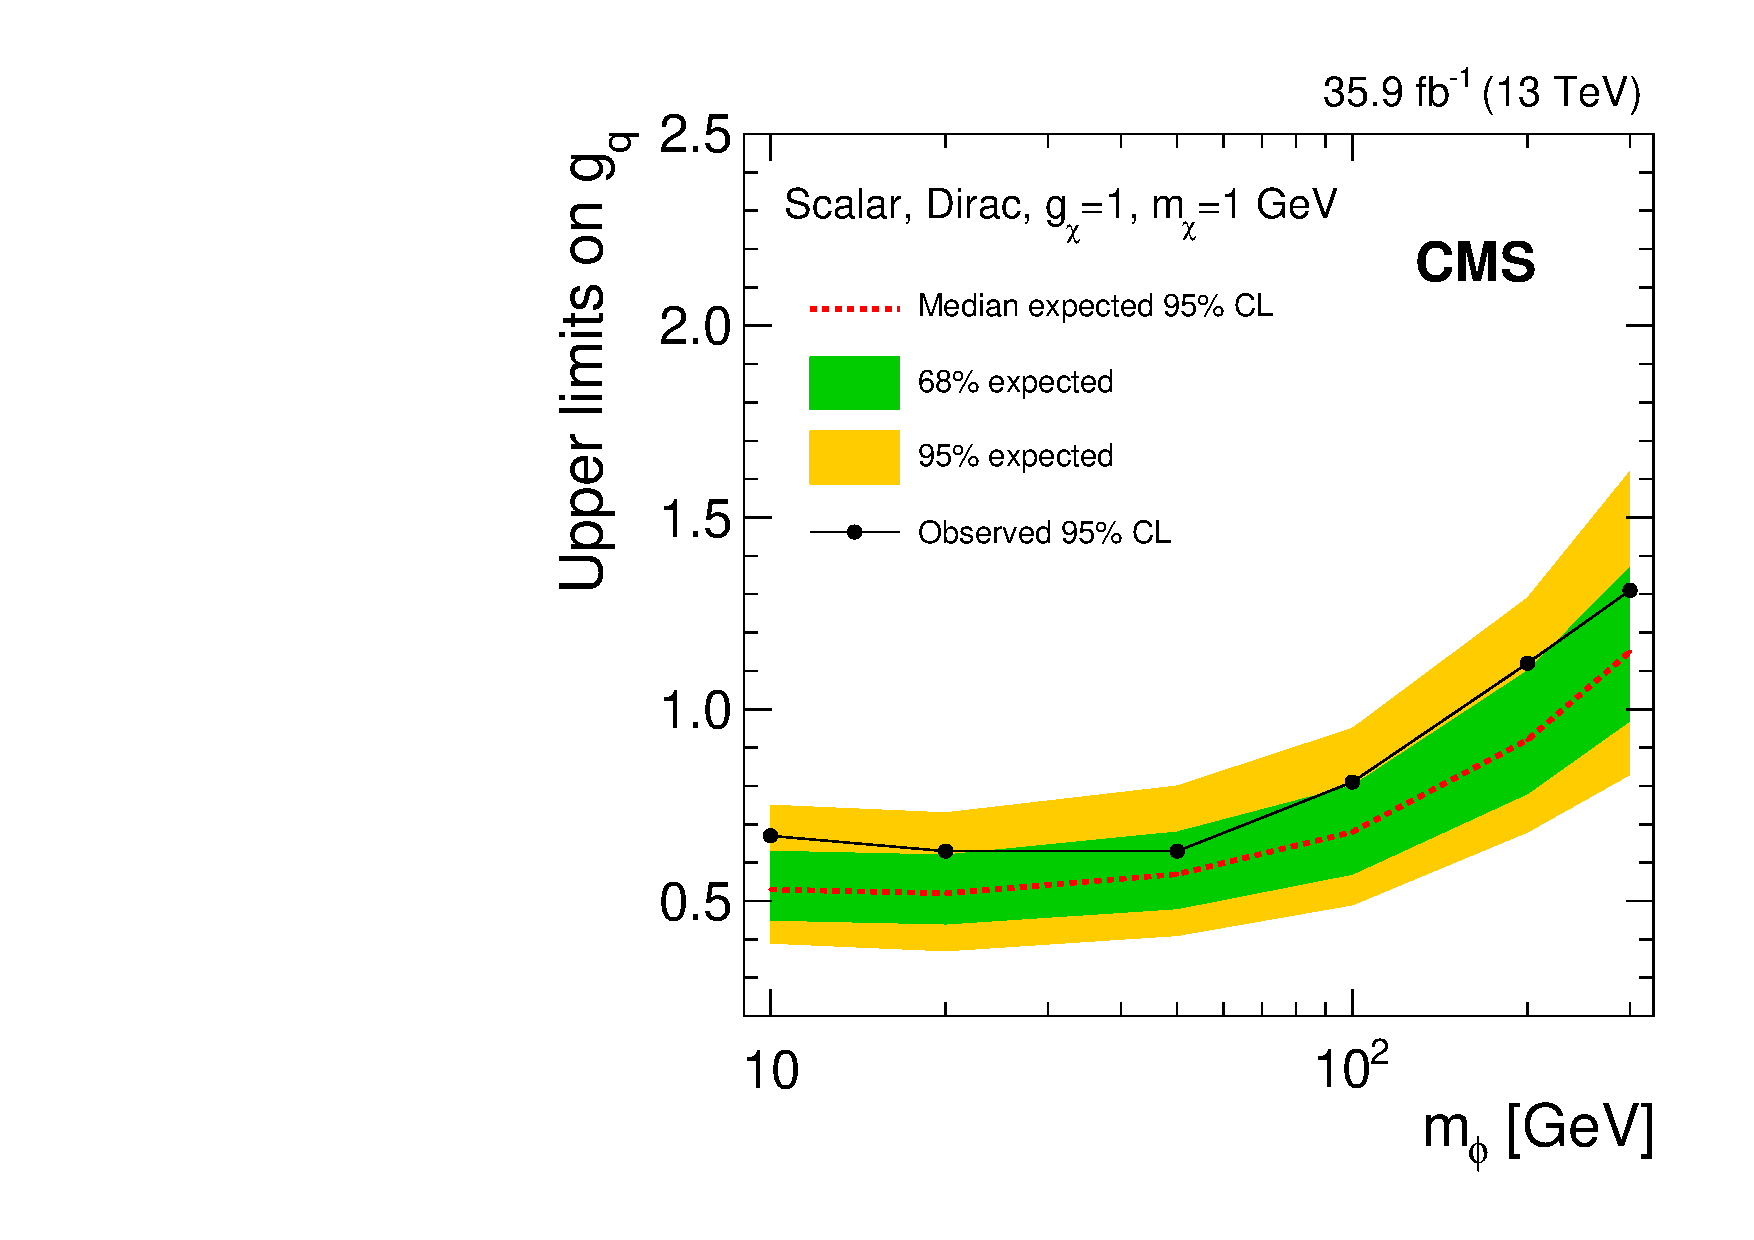
\includegraphics[height=7.3cm]{fig/CMS-EXO-16-049_Figure_003-a.pdf}
\caption{Masa invariante de dos leptones: comparación entre datos observados y predicciones de fondo (izquierda). Límites superiores observados y esperados, con nivel de confianza del 95\%, en la constante de acoplamiento de un mediador de Materia Oscura escalar al quark top (derecha).} 
\label{fig:edge}
\end{figure} 



\paragraph{Desarrollo de triggers y de simulaciones para el grupo de SUSY de CMS\\\\}

Durante los años 2014-2016 fui seleccionado por el grupo de SUSY de CMS como el co-coordinador (L3) del grupo de \emph{SUSY Trigger, Montecarlo and Interpretations}. Mis responsabilidades en este ámbito pasaban fundamentalmente por la coordinación del diseño de las estrategias de trigger y de simulación de Monte Carlo de todos los análisis de SUSY dentro de CMS y de cara a la toma de datos del año 2016, la primera con una energía del centro de masas de $\sqrt{s}=$ 13~TeV. En este contexto, también era el responsable de defender los intereses del grupo de SUSY dentro de los correspondientes grupos de Trigger y Simulación en la colaboración. Este trabajo me permitió adquirir una visión global y privilegiada del grupo, al trabajar de forma conjunta con todos los equipos de análisis, siendo en la mayor parte de los casos yo mismo el que implementaba técnicamente los triggers dentro del sistema de trigger de CMS, o el encargado de generar las simulaciones, especialmente en el caso de procesos de señal. En el año 2016, fui invitado por la colaboración CMS para mostrar los primeros resultados de SUSY de la historia, a una energía de $\sqrt{s}$=13~TeV, en el prestigioso \emph{LHC seminar}. También fui organizador de los \emph{CMS SUSY Workshops} de 2014 y 2015 en Lisboa y Chicago respectivamente y editor del capítulo de SUSY del artículo de trigger de CMS~\cite{Trigger}.


\paragraph{Búsquedas de partículas supersimétricas de tercera generación\\\\}

A finales del año 2016, con mi inminente incorporación al Instituto de Física de Cantabria (IFCA) comencé a trabajar en una búsqueda de producción directa de charginos y stops en sucesos con dos leptones de diferente sabor y carga contraria~\cite{Luca}, que fue íntegramente realizado por miembros del IFCA. También hice contribuciones a una búsqueda de producción directa de stops en el régimen en el que la masa del stop es próxima a la masa del quark top~\cite{Oviedo}, haciendo que la topología final disponga de escaso momento transverso faltante. Durante los años 2016 a 2018 fui seleccionado como co-coordinador (L3) del grupo de búsquedas de partículas supersimétricas de tercera generación, estando bajo mi responsabilidad la mejora, escrutinio y aprobado de este tipo de búsquedas, así como el diseño de la estrategia global del grupo y la combinación de los diferentes sub-análisis. En este papel, fui parte del comité científico organizador de los “CMS SUSY Workshops” de  2017 en Gante y 2018 en Viena. En el año 2019 la colaboración CMS me encomendó también la organización del “CMS SUSY Workshop” en Santander.


\paragraph{Búsquedas directas de Materia Oscura\\\\}

Entre los años 2017 y 2018 lideré en el IFCA una búsqueda de materia oscura en asociación con pares de quark top-antitop~\cite{TopDM}. En este análisis desarrollé un método para estimar el momento transverso del mediador de materia oscura. Esta búsqueda dio lugar a una tesis doctoral de la cuál fui co-director y a dos trabajos de fin de grado: uno sobre una extensión analítica para calcular el momento transverso del mediador, y otro sobre una aplicación de un \emph{Variational Autoencoder} para la producción de simulaciones de MC realistas partiendo de sucesos reales. La Fig.~\ref{fig:edge} muestra los límites superiores a la constante de acoplamiento de un mediador de materia oscura al quark top, obtenidos en el análisis. En el año 2019, presenté el resumen de resultados de materia oscura de CMS en una charla plenaria en los “LHC Split Days” en Croacia. Posteriormente y hasta la actualidad, he seguido liderando en el IFCA una nueva búsqueda de materia oscura en asociación con quarks top, incluyendo todos los datos del Run 2 y nuevos modelos con producción de “single-top”. Este hecho ha requerido una intensa investigación para añadir zonas de señal con menor multiplicidad de jets. Dos métodos de aprendizaje automático (Redes Neuronales y \emph{Boosted Decision Trees}) están siendo utilizados para mejorar la discriminación de señal. El análisis está siendo realizado en colaboración con DESY y  la Universidad de Winsconsin-Madison, y se espera que sea público en los próximos meses. Este trabajo está dando lugar también a otra tesis doctoral de la que soy co-director. Como una mejora adicional al método de estimación del momento transverso del mediador de materia oscura, también dirigí un TFG en el que la estimación era realizada por una red neuronal en modo regresión, y otro TFG estudiando el efecto de los errores sistemáticos en la respuesta de una red neuronal discriminadora. Ambos resultados fueron presentados en la conferencia \emph{10th International Conference on New Frontiers in Physics (ICNFP 2021)}.

\paragraph{Producción de partículas con larga vida media\\\\}

En el año 2018, en el contexto del \emph{Technical Design Report} (TDR) del MIPs Timing Detector (MTD)~\cite{MTDTDR} de CMS, desarrollé una búsqueda de leptones desplazados que tenía como objetivo demostrar las posibilidades únicas que el MTD proporciona para discriminar los leptones desplazados en base a su retraso, y también para medir la masa de la partícula de larga vida media utilizando la medida de su velocidad, estimada a través de la posición y tiempo del vértice desplazado con respecto al primario. El estudio fue incluído en el TDR del MTD y se convirtió en uno de los estudios de referencia para dicho sub-detector. Adicionalmente, en 2019 comencé a desarrollar una búsqueda de partículas con larga vida media dando lugar a pares de leptones desplazados. Estas búsquedas son del máximo interés, dada la aparente ausencia de Nueva Física en las topologías convencionales. Actualmente me encuentro co-dirigiendo una tesis doctoral en este tema. Las novedades de este análisis incluyen el diseño de nuevos objetos tanto de electrones como de muones desplazados que han sido adoptados como nuevos estándares por parte de los grupos de muones y \emph{e-gamma} de CMS respectivamente. El análisis comenzará en breve el escrutinio interno de CMS, tras haber sido presentado en los \emph{EXO workshops} de CMS en 2019 en Aachen y de 2020 (virtual).

\paragraph{Producción de pares de bosones de Higgs\\\\}

En el año 2018, fui nombrado co-coordinador (L3) del sub-grupo de Física del \emph{Data Performance Group (DPG)} del MTD, siendo responsable de elaborar una serie de análisis en donde se pudiese observar de forma clara y evidente el potencial del MTD y su impacto en el programa de Física de CMS para el HL-LHC. Una descripción más detallada sobre este papel puede encontrarse en~\ref{MTDFisica}. En este contexto, estuve a cargo de coordinar a los cuatro equipos de investigación que trabajaban en el análisis de la medida de la sección eficaz del proceso de producción de pares de bosones de Higgs, en los cuatro canales estudiados $HH\rightarrow b\bar{b}b\bar{b}$, $HH\rightarrow b\bar{b}\gamma\gamma$, $HH\rightarrow b\bar{b}\tau\tau$, $HH\rightarrow b\bar{b}W^{+}W^{-}$, $HH\rightarrow b\bar{b}ZZ$. El análisis suponía una proyección de la significancia estadística con la que podía observarse el proceso proyectando al total de la luminosidad integrada que se espera que recoja el HL-LHC. Mi papel tuvo que ver con la implementación de las mejoras producidas por el uso del MTD en los diferentes objetos físicos. También estuve a cargo de la combinación y fui editor de la nota interna de CMS que describía el análisis, así como el encargado de defenderlo frente a la colaboración.


\subsection{Búsquedas de Nueva Física con datos del Run 3 en CMS}

El Run 3 del LHC comenzará en el año 2022 y se extenderá hasta el año 2024, recogiendo una cantidad de datos esperada de 160~fb$^{-1}$, a una energía del centro de masas aún por determinar y que estará en el rango $\sqrt{s}$=13-14~TeV. Esta línea de investigación persigue extender y optimizar las búsquedas previas con especial énfasis en las zonas del espacio de parámetros de los modelos con una sensitividad reducida.  

\paragraph{Búsqueda de SUSY con dos leptones del mismo sabor y carga opuesta\\\\}

Este análisis supone una extensión de los análisis previos usando toda la luminosidad del Run 3. La búsqueda es particularmente relevante si la energía del centro de masas del acelerador se incrementa, ya que el análisis buscaría la aparición de estructuras en la masa invariante de los dos leptones a dicha energía sin precedentes, constituyendo una de las búsquedas esenciales de la colaboración. En cualquier caso, la búsqueda será optimizada para aquellos modelos de sección eficaz más baja, como son la producción directa de sleptons o la producción de charginos y neutralinos, en donde los límites superiores establecidos hasta ahora en el LHC aún tienen margen de mejora. Las últimas medidas del factor \emph{g-2} motivan fuertemente las búsquedas de sleptons ya que éstas favorecen la existencia de sleptons con masas en el rango del TeV. 

El análisis contará con varias mejoras técnicas para aumentar su sensitividad a la Nueva Física. En primer lugar, se estudiará el uso de nuevos triggers de dileptones de CMS, que usando mejoras como la inclusión del algoritmo \emph{Kalman-Filter}~\cite{bib:kalman} en el trigger L1, podrían reducir los umbrales del momento transverso de los leptones, aumentando la sensitividad a modelos con espectro comprimido. La Fig.~\ref{fig:slepton} muestra los límites superiores en la sección eficaz de producción de pares de sleptons y de producción directa de charginos y neutralinos. Las diagonales son zonas de baja sensitividad debido a que la escasa diferencia de masa entre sleptons (neutralinos/charginos) y los neutralinos más ligeros, hace que los leptones en el estado final sean muy poco energéticos y no pasen el umbral de trigger. En esta misma línea, se añadirán también zonas de señal que incluyan un jet muy energético de tipo \emph{Ìnitial State Radiation}, provocando un \emph{boost} del sistema del par de partículas supersimétricas e incrementando así su momento transverso. El objetivo final será explorar la existencia de partículas supersimétricas en configuraciones de espectro de masas comprimidos.

\begin{figure}[ht]
\centering
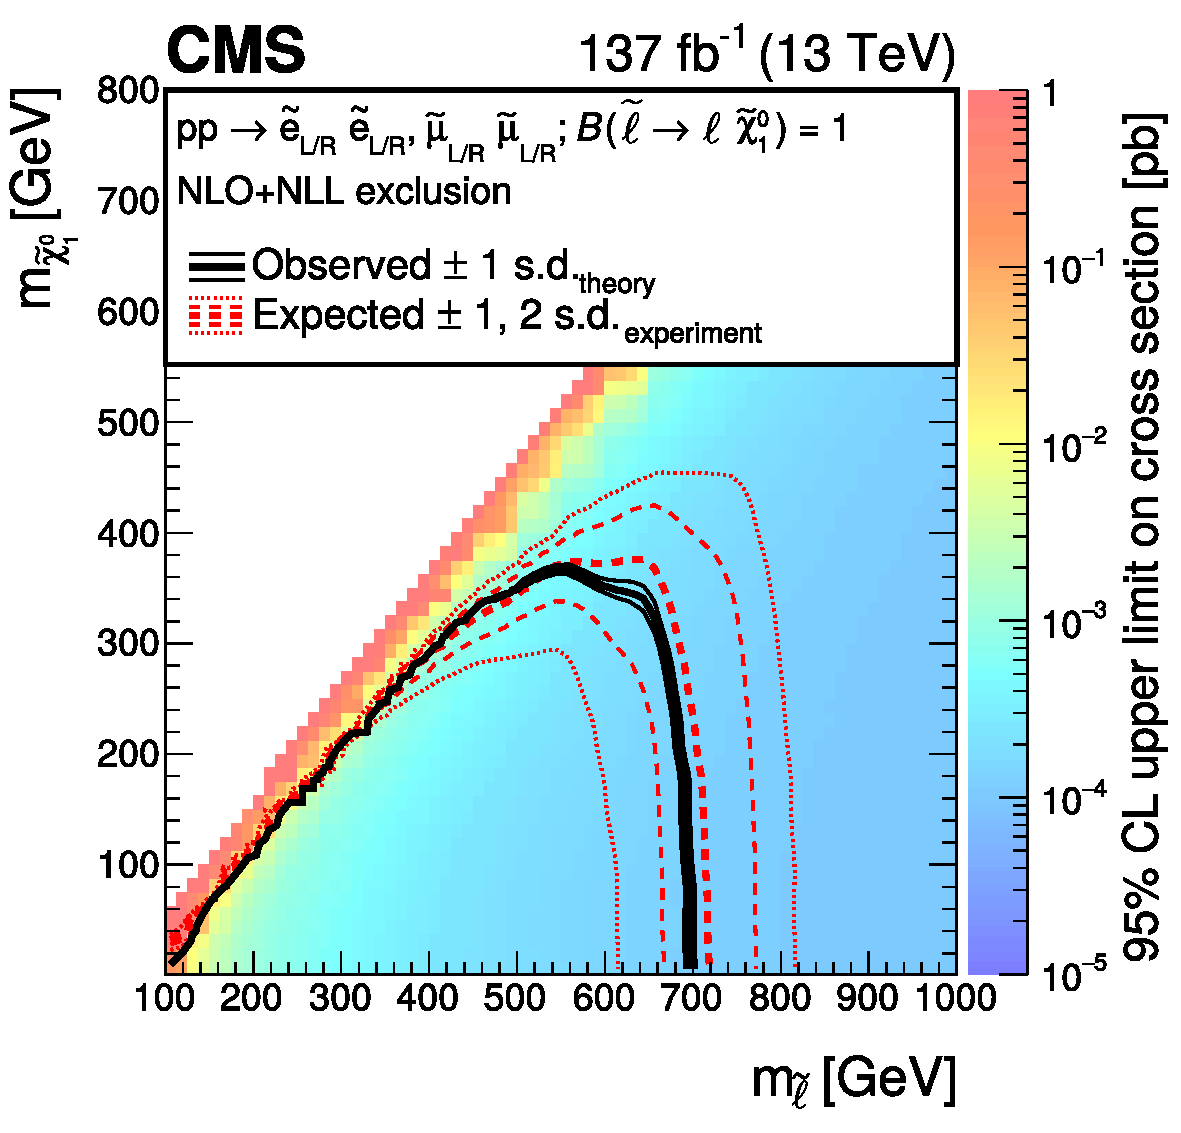
\includegraphics[height=7.3cm]{fig/CMS-SUS-20-001_Figure_014.pdf}
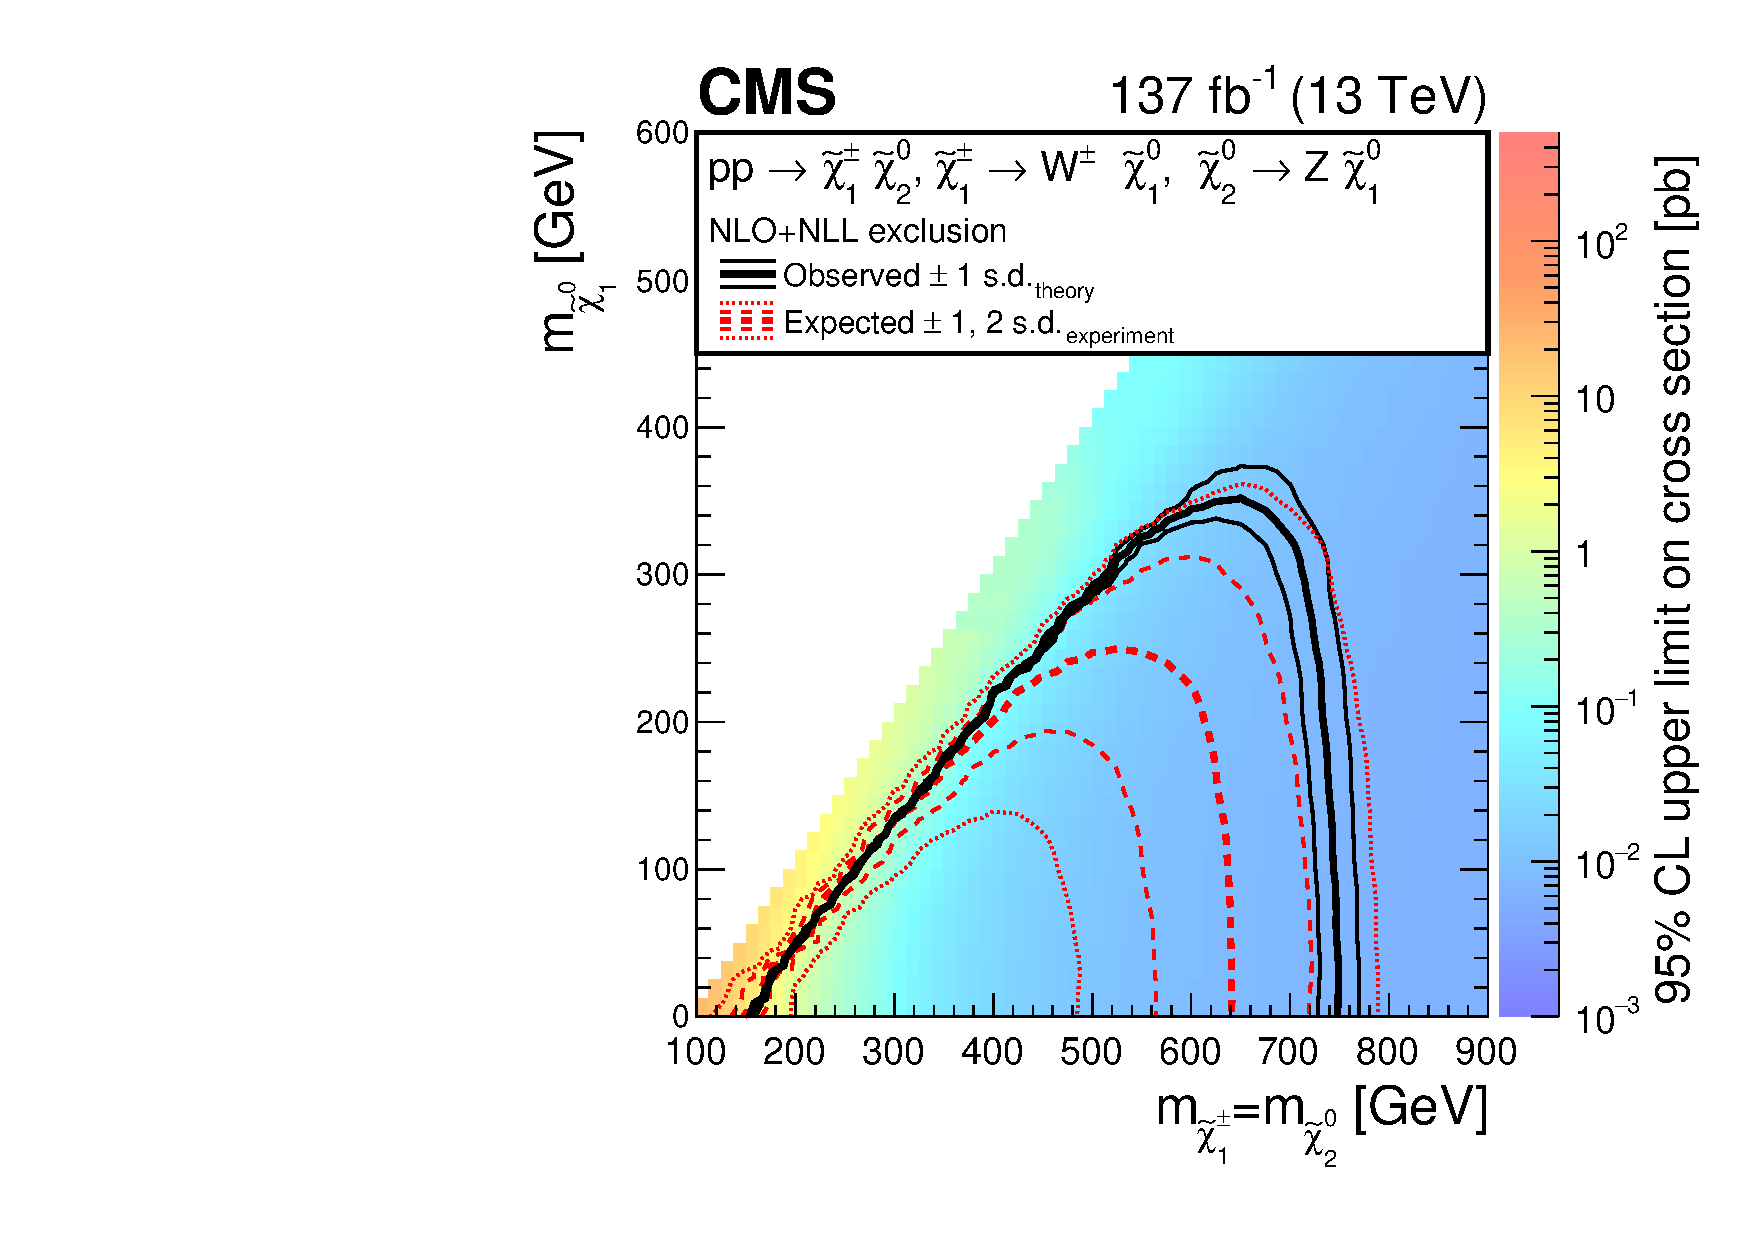
\includegraphics[height=7.3cm]{fig/CMS-SUS-20-001_Figure_011.pdf}
\caption{Límites superiores en la sección eficaz de producción de pares de sleptons en función de su masa y de la masa de los neutralinos a los que decae (iqzuierda). Límites superiores en la sección eficaz de producción de charginos y neutralinos en función de su masa y de la masa del neutralino más ligero al que decaen (derecha).}
\label{fig:slepton}
\end{figure} 

En segundo lugar, se explorará el uso de algoritmos de aprendizaje automático para caracterizar la presencia de bosones W decayendo a jets en los sucesos. La sensitividad de las búsquedas de producción de charginos y neutralinos está limitada en la zona de alta masa (ver Fig.~\ref{fig:slepton}, derecha), por el hecho de que el bosón W adquiere suficiente momento como para que los dos jets producto de su desintegración se fundan en uno solo. En versiones anteriores del análisis se introdujeron zonas de señal utilizando \emph{fat jets} y obteniéndose una mejora sustancial. En el Run 3 se utilizarán métodos de aprendizaje automático (taggers) para determinar a través de la sub-estructura, si un jet proviene de la desintegración de un W de alto momento.

\paragraph{Búsqueda de materia oscura en asociación con top quark(s)\\\\}

Este análisis constituye también una extensión y optimización del análisis llevado a cabo con los datos del Run 2. La búsqueda de materia oscura sigue constituyendo uno de los ejes del programa de física del LHC, y su producción en asociación con el quark top tiene una gran relevancia, debido a la singular relación del quark top y el sector del bosón de Higgs.

Existen tres nuevos desarrollos de gran calado en el análisis. En primer lugar, el análisis del Run 3 no se limitará al canal dileptónico, sino que también se llevará a cabo el canal semileptónico, en el que uno de los W decae hadrónicamente. El grupo encargado de realizar la versión semi-leptónica del análisis en el Run 2 ha demostrado grandes dificultades para desarrollar la búsqueda, así que, se procederá a la colaboración con dicho grupo para realizar esa parte del análisis que constituye una parte importante de la sensitividad total al modelo. En segundo lugar, se va a potenciar el uso de \emph{taggers} basados en algoritmos de aprendizaje automático para identificar la presencia de decaimientos de quarks top o bosones W de alto momento, dando lugar a un sólo jet que no puede ser resuelto como la unión de dos o tres jets. 

El último elemento novedoso, surge de las investigaciones realizadas recientemente en un TFG dirigido por mí, en el que se investigaba la posibilidad de predecir el momento transverso del mediador de materia oscura utilizando una red neuronal en modo regresión. El método demostró un mejor desempeño que las versiones numérica y análitica desarrolladas previamente. Además, el método permite estimar también el momento transverso del mediador en el caso de los modelos con presencia de un único quark top. La información del momento del mediador será utilizada para mejorar la discriminación señal-fondo en el contexto del análisis. 

\paragraph{Búsqueda de partículas de larga vida media decayendo a pares de leptones\\\\}

Los resultados del Run 2 del LHC no han mostrado evidencias de Nueva Física. Una de las posibles explicaciones consiste en que la Nueva Física aparezca en topologías para las que los detectores no fueron optimizados y que por tanto son difíciles de reconstruir. Los modelos con partículas de larga vida media entran dentro de esta categoría ya que los productos de su desintegración ocurren alejados del centro del detector, confundiendo a los algoritmos de reconstrucción, en general optimizados para reconstruir partículas que provienen del punto de interacción. Este análisis propone una búsqueda similar a la ejecutada en el Run 2, en el que una interacción mediada por un bosón de Higgs produce dos bosones con largo tiempo de vida que decaen en pares de leptones desplazados. La búsqueda también considera la exploración de un modelo de Supersimetría con \emph{violación de la paridad-R}, en el que dos stops con larga vida media decaen a dos leptones del mismo sabor y un neutrino. 

Una de las grandes complicaciones relacionadas con esta búsqueda en el Run 2 tuvo que ver con la ausencia o ineficiencia de los triggers de leptones desplazados. Uno de los objetivos para el Run 3 consiste en la exploración y estudio de nuevos triggers para este tipo de objetos. En el caso de los muones se pretende utilizar el nuevo algoritmo de Kalman-Filter en el nivel L1 del trigger para desarrollar nuevos triggers en el High Level Trigger que maximicen la sensitividad de la búsqueda. Los desarrollos llevados a cabo en el análisis del Run 2 para conseguir un nuevo objeto de muon desplazado serán implementados a nivel de trigger para intentar reducir los umbrales de momento de los leptones, aumentando de esta manera la sensitividad a modelos comprimidos en los que los leptones son de bajo momento. Una colaboración con miembros de la Universidad de Oviedo ha sido iniciada en la actualidad para perseguir este objetivo. 

\subsection{Búsqueda de Nueva Física en el HL-LHC}

El HL-LHC que comenzará en los próximos años recogerá una cantidad de datos sin precedentes, $L_{int}=3000~fb^{-1}$, durante sus años de operación. Por otro lado, sus condiciones de operación serán extremadamente complejas fundamentalmente debido al alto número de colisiones simultáneas \emph{pile-up} que tendrán lugar en cada \emph{bunch-crossing} entre los haces de protones. Si durante el Run 2 del LHC el nivel medio de pile-up estuvo en torno a 40-50, en el HL-LHC este valor aumentará hasta 200. El incremento masivo del número de \emph{hits} en el tracker de CMS complicará enormemente la reconstrucción de trazas y la identificación del vértice primario, haciendo que el análisis de datos sea un reto en muchos casos. El nuevo detector MTD tiene como objetivo reducir el impacto del pile-up ayudando a reducir sus niveles a valores parecidos a los del LHC. La segunda línea de investigación presentada en este proyecto tiene que ver con mi participación en el proyecto del MTD. La experiencia adquirida en ese contexto será utilizada para conseguir una posición de liderazgo en el análisis de datos del HL-LHC. Concretamente se perseguirá realizar un gran impacto en dos tipos de análisis en los que el MTD ha demostrado ofrecer ventajas sustanciales: búsquedas de partículas con larga vida media y la búsqueda de la producción de pares de bosones de Higgs.

\paragraph{Búsqueda de partículas de larga vida media en el HL-LHC\\\\}

El objetivo de este análisis consiste en mejorar la sensitividad del experimento CMS a modelos de Nueva Física con leptones desplazados. Si el análisis del Run 3 tuvo éxito encontrando indicios de la existencia de nuevas partículas con larga vida media, éste análisis incidirá en la medida detallada de sus propiedades. Si por el contrario, el análisis del Run 3 no arrojó ningún resultado positivo, este análisis extenderá la búsqueda aprovechando la gran cantidad de datos proporcionada por el HL-LHC. 

Para llevar a cabo esta tarea, se utilizará la información temporal proporcionada por el MTD para discriminar e identificar las posibles partículas desplazadas, prestando atención al retraso temporal que sufrirán si fueron producidas por una partícula de larga vida media y muy masiva. Tal y como mostré en el TDR del MTD, en algunos modelos, resulta posible incluso reconstruir la masa de las partículas de larga vida calculando su velocidad $\beta$ a través de la diferencia temporal entre el vértice desplazado y el vértice primario y su distancia. Este tipo de análisis supondría una potente herramienta para estudiar posibles modelos de Nueva Física. 

\paragraph{Análisis de la producción de pares de bosones de Higgs en el HL-LHC\\\\}

Este análisis constituye uno de los principales elementos del programa de física del HL-LHC. La producción de pares de bosones de Higgs aporta información sobre el acoplamiento triple, \emph{trilinear coupling}, del potencial de Higgs y por lo tanto constituye una prueba fundamental del mecanismo de ruptura de simetría propuesto por Higgs. La sección eficaz de este proceso tiene una alta sensitividad a modelos de Nueva Física como por ejemplo aquellos que incluyen \emph{Higgs compuestos} o \emph{Higgs portal} y por lo tanto su estudio es de una importancia capital también en el contexto de las búsquedas. El detector MTD eligió esta análisis como campo de pruebas en el que demostrar su impacto. 

La propuesta de este proyecto consiste en aprovechar el conocimiento adquirido trabajando en el MTD para liderar uno de los canales asociados a este análisis: el caso en el que uno de los bosones de Higgs decae a un par de quarks bottom-antibottom, y el otro a dos bosones W ($HH\rightarrow b\bar{b}W^+W^-$) con los W decayendo semi-leptónicamente a leptón (electrón o muon) y neutrino. El ingrediente principal de este análisis consiste en aprovechar la información temporal proporcionada por el MTD para desechar trazas espúreas del cono de aislamiento de electrones y muones, proporcionando así una selección de \emph{aislamiento} mucho más eficiente, reduciendo también dramáticamente el número de leptones erróneamente reconstruidos como tales.


\section{Participación en el ``Phase 2 Upgrade'': el MTD}

Esta línea de investigación consiste en la participación en el proyecto de \emph{Phase 2 Upgrade} de CMS de cara a su puesta a punto para operar bajo las exigentes condiciones del HL-LHC. Concretamente la línea discurrirá en el contexto del \emph{MIPs Timing Detector} (MTD), un nuevo detector que será instalado a continuación del tracker de CMS y con capacidad para medir el tiempo de paso de las partículas cargadas con una precisión inicial de 35-40~ps al inicio del HL-LHC y de unos 60~ps al final de su tiempo de vida. El MTD será extremademente útil para mitigar los efectos negativos del alto \emph{pile-up} con el que el HL-LHC operará, y por lo tanto tendrá un impacto integral en el programa de Física de CMS. El trabajo propuesto se ocupará de dos líneas de actuación: el desarrollo del software de simulación, reconstrucción, calibración y alineamiento del detector; y el ensamblado de los módulos del \emph{Endcap Timing Layer (ETL)} del MTD.

\subsection{Experiencia previa}

\paragraph{Física con el MTD\\\\}\label{MTDFisica}

Comencé a trabajar en el proyecto del MTD en el año 2017 cuando me incorporé al Instituto de Física de Cantabria. Mi primera contribución fue el desarrollo de un búsqueda de Nueva Física en un estado final con leptones deplazados, aprovechando la información temporal proporcionada por el MTD para discriminar sucesos de señal de sucesos de fondo. Un resumen más detallado sobre este análisis se proporcionó en la sección anterior. En el año 2018, fui nombrado coordinador del sub-grupo de Física del \emph{Data Performance Group (DPG)} del MTD, siendo responsable de elaborar una serie de análisis en donde se pudiese observar de forma clara y evidente el potencial del MTD y su impacto en el programa de Física de CMS para el HL-LHC. En este contexto y además del análisis mencionado anteriormente, coordiné y participé en otras búsquedas de Nueva Física usando el MTD, como por ejemplo, la búsqueda de fotones desplazados, de jets desplazados, o también de búsquedas de \emph{Heavy Stable Charged Particles (HSCP)}. Paralelamente también estuve a cargo de coordinar a los cuatro equipos de investigación que trabajaban en el análisis de la medida de la sección eficaz del proceso de producción de Higgs doble, tal y como se explicó en la sección anterior. Todos estos análisis fueron recogidos en dos notas internas de la colaboración de las que fui editor y que tuve que defender dentro del grupo correspondiente del Upgrade para que los resultados fueran aprobados. Finalmente, todos los análisis fueron includios en el TDR del MTD constituyendo su justificación como proyecto desde el punto de vista físico. También fui editor del capítulo correspondiente del TDR.

\paragraph{``L1 Trigger'' usando el MTD\\\\}

En el año 2018, el grupo de upgrade de CMS en conjunto con el MTD y el grupo de \emph{Trigger L1} para el upgrade, me encomendaron la tarea de elaborar un estudio detallado sobre el impacto de incluir la información del MTD a nivel de trigger L1. Mis estudios mostraron un análisis exhaustivo de todos los posibles usos que podían darse de la información del MTD para elaborar \emph{L1 seeds}, así como de ejemplos de análisis y búsquedas que pudieran beneficiarse de las mismas. Los resultados mostraron que las mejoras observadas no eran muy significativas en relación con el uso del MTD en el proceso de reconstrucción normal. Mis resultados fueron presentados por mí en dos workshops específicos del Upgrade de CMS y resultaron fundamentales para la decisión final adoptada por los grupos de Upgrade y del MTD de no incluir la información del MTD a nivel de trigger.     

\paragraph{Simulación, reconstrucción, calibración y alineamiento del MTD\\\\}

En septiembre del año 2019 fui elegido como co-coordinador (L2) del DPG del MTD. Como tal, estoy a cargo de la implementación de las geometrías del MTD en el software oficial de CMS, así como de los algoritmos de simulación, digitización, reconstrucción, cálculo de vértices, calibración, alineamiento y también del estudio de la mejora de los objetos de física tras la inclusión del MTD. Entre otros desarrollos, recientemente he llevado a cabo la integración del MTD en el sistema de “navegación” de CMS, de manera que los algoritmos de
reconstrucción se extienden de manera natural al uso del MTD, o también los primeros pasos de la implementación de una simulación realista para la \emph{digitización} de los sensores LGAD dentro del software de CMS. También he defendido las actuaciones del DPG en el “Annual Review” del proyecto ante el correspondiente comité de CMS (8 de octubre de 2020) y también he presentado el proyecto en conferencias como Lepton Photon 2019 o LHCP20. En el año 2021, el grupo del MTD decidió re-elegirme durante 2 años más como co-coordinador del DPG del MTD.

\paragraph{Ensamblado de los módulos del ETL\\\\}

Dentro del proyecto de instrumentación del grupo de Altas Energías del Instituto de Física de Cantabria, soy el responsable del ensamblado de los módulos del Endcap Timing Layer del MTD. El IFCA ha adquirido el compromiso de ensamblar un total de aproximadamente 900 módulos del ETL. La figura~\ref{fig:etl} muestra un esquema de la estructura general del ETL (izquierda) y del diseño de los módulos que lo componen. Dento de los módulos los conponentes más importantes son el sensor LGAD y los módulos de electrónica (ETROC). 

\begin{figure}[ht]
\centering
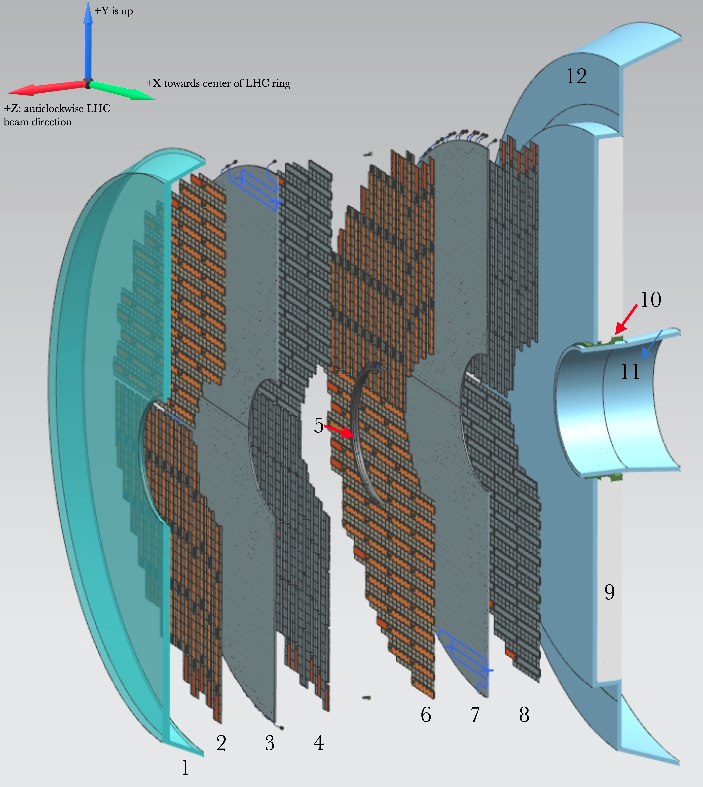
\includegraphics[height=5.3cm]{fig/etloverview.png}
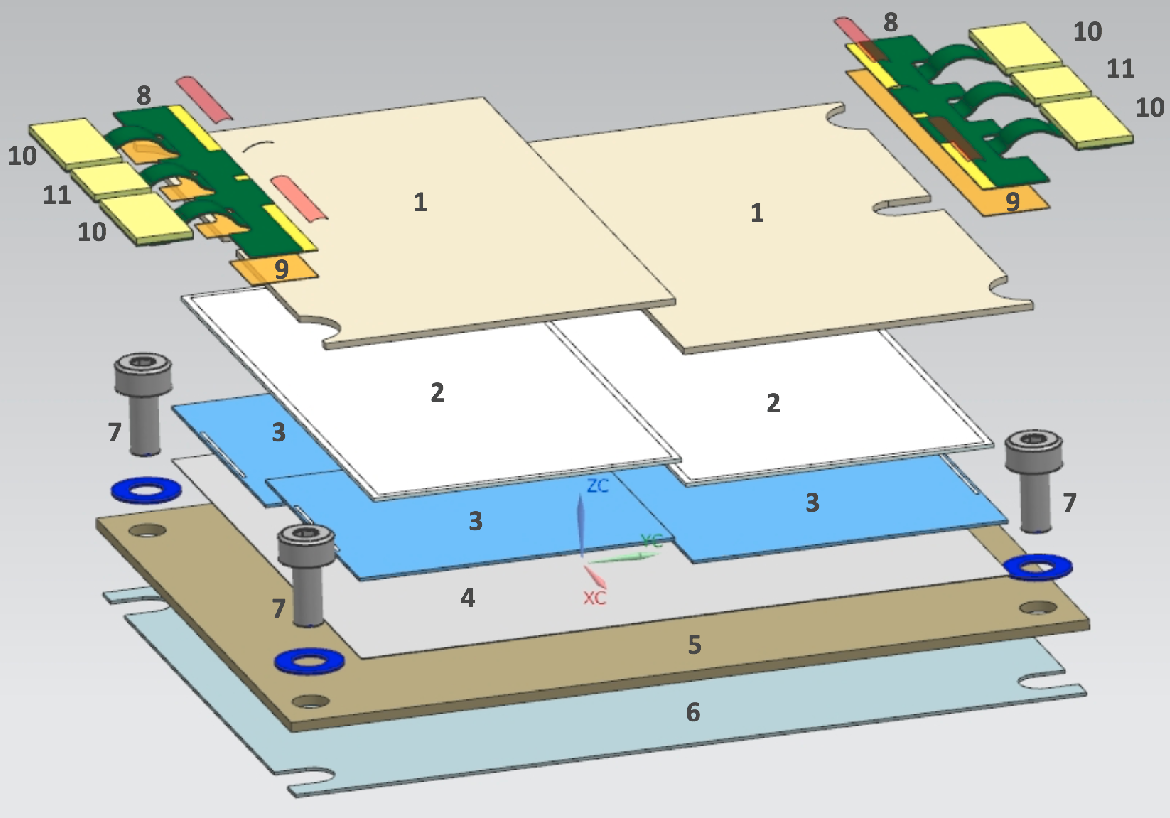
\includegraphics[height=5.3cm]{fig/etlmodule.png}
\caption{Esquema general del ETL del MTD (izquierda) y esquema de un módulo del ETL incluyendo las diferentes capas que lo conforman (derecha).}
\label{fig:etl}
\end{figure} 

El ensamblado de los módulos del ETL será realizado de forma automática con ayuda de un robot de posicionamiento. Durante los años 2020 y 2021 he dirigido un Trabajo de Fin de Grado y un Trabajo de Fin de Máster con objeto de realizar el \emph{commissioning} de un robot de posicionamiento disponible en las instalaciones del IFCA, así como dar los primeros pasos en su programación, utilizando un lenguaje dedicado conocido como V+.  

\subsection{Desarrollo del software del MTD}

En septiembre del año 2021 fui reelegido como co-coordinador (L2) del Data Performance Group del MTD por un periodo de dos años. En este tiempo lideraré un programa completo de desarrollos que tendrán como objetivo poner los pilares básicos de la infraestructura de software del detector MTD. En este sentido se identifican varios actividades que serán acometidas por parte del DPG y que se describen a continuación.

\paragraph{Software de ``digitización'' del ETL\\\\}

El software de digitización está encargado de simular la respuesta de los sensores y de los módulos electrónicos de lectura. En el caso del ETL, el software de digitización es una simple traducción de los llamados \emph{SimHits} proporcionados por GEANT4~\cite{geant4} en términos de coordenadas locales de activación dentro del sensor. Los desarrollos llevados a cabo por mí en los últimos meses, implementaron de manera lógica los píxeles dentro de los sensores LGADs, así como las zonas de no-ganancia entre píxeles. No obstante, una simulación realista del proceso de medida requiere parametrizar la forma de la señal obtenida en el sensor en función de la energía, posición y dirección de los SimHits. Dicha forma de señal tiene que ser entonces transformada por la acción esperada que los módulos electrónicos de lectura ejerzan sobre ella. En la actualidad, me encuentro personalmente comenzando este esfuerzo en comunicación con los expertos en electrónica del ETL y con ayuda de un estudiante en el IFCA.     

\paragraph{Integración del MTD en el tracking de CMS\\\\}

La información temporal proporcionada por el MTD debe ser asignada a las trazas reconstruidas por el tracker de CMS y propagada hacia el punto de interacción para determinar el tiempo asociado a dicha traza en el origen. Puesto que el MTD añade de manera lógica nuevas capas al tracker de CMS, resulta conveniente extender toda la infraestructura de reconstrucción de trazas para que sea capaz de incorporar y reconocer al MTD. La primera acción en esta dirección fue realizada por mí en el año 2020, modificando la estructura de navegación del software de CMS, para que los algoritmos de reconstrucción sean capaces de incorporar información de las capas correspondientes al MTD. El siguiente paso consiste en la adaptación de las estructuras utilizadas por el algoritmo de Kalman-Filter para que pueda usar de forma efectiva la información aportada por el MTD. A continuación, será necesario integrar la propagación de la información temporal al punto de origen. Este proceso de propagación requiere hacer una hipótesis acerca de la masa de la partícula generadora de la traza. Encontrar un método para elegir la masa correcta a partir de la información disponible tanto en la traza como en el MTD, constituye otro desafío que será acometido en este punto. Las modificaciones resultantes deberán ser, además, integradas dentro del contexto del tracking iterativo de CMS. Todos estos desarrollos serán realizados personalmente por mí con ayuda de expertos de tracking de la colaboración CMS. 

\paragraph{Reconstrucción de vértices utilizando información temporal\\\\}

Una vez las trazas han sido provistas de un tiempo de generación en el origen, es posible utilizar dicha información para ayudar a reconstruir los vértices. Un primer intento fue llevado a cabo en el momento en el que se configuró el TDR. La aproximación consistió en extender el algoritmo estándar de reconstrucción de vértices de CMS basado en el concepto de \emph{Deterministic Annealing} para que usase no sólo la información espacial longitudinal de las trazas sino también su tiempo de producción. Investigaciones posteriores al TDR han mostrado que los resultados de este algoritmo no son capaces de mejorar el desempeño del algoritmo clásico que utiliza únicamente la información espacial. Esta inconsistencia está siendo objeto de una intensa investigación por parte de expertos en reconstrucción de vértices y con la supervisión de los co-coordinadores del MTD. Si el problema no llega a resolverse en los próximos meses, se explorarán mecanismos alternativos, como puede ser el uso inicial de la información espacial para el \emph{Deterministic Annealing}, y un segundo paso de refinamiento que utilice la información temporal para limpiar los vértices obtenidos de trazas espúreas. 

\paragraph{Calibración y alineamiento del MTD\\\\}

El MTD requiere de una infraestructura de software que permita calibrar sus componentes. El diseño de esta infraestructura parte en primer lugar de la identificación del total de constantes y calibraciones necesarias por los sistemas. En segundo lugar han de definirse los procedimientos para estimar dichas constantes y determinar la frecuencia con la que han de ser calculadas. Es preciso también disponer de una infraestructura de base de datos en las que las constantes puedan ser almacenadas con atención a los rangos de validez de cada conjunto de calibraciones. Finalmente, el software del detector tiene que ser capaz de de leer y aplicar las calibraciones para proporcionar una respuesta óptima del detector. De la misma forma, el detector requiere también un conjunto de procedimientos que permitan alinear sus componentes. Además de los algoritmos de alineamiento es preciso dotar al detector de una infraestructura de software que permita implementar las correcciones de alineamiento así como dar cuenta de los errores de posicionamiento asociados. Todas estas actividades serán llevadas a cabo en los años venideros, lideradas por los co-coordinadores del DPG. 

\paragraph{Desempeño del detector y ``Physics case''\\\\}

Todos los desarrollos de software acometidos en el detector han de tener como consecuencia la mejora de la reconstrucción de los diferentes objetos físicos. El DPG ha de garantizar que toda la información relevante está disponible en los diferentes formatos de datos de CMS. El DPG ha de proporcionar también todo el soporte necesario a los grupos dedicados a los diferentes objetos de física para que la nueva información temporal sea aplicada de forma afectiva. Durante los próximos años se espera un diálogo constante con estos grupos en el que aparezcan ideas acerca de cómo dar mejores usos a la información temporal y de cómo medir la eficacia de los objetivos conseguidos. De igual manera, durante los próximos años se buscará ampliar la gama de análisis de física en los que el MTD tenga un papel determinante. Las ideas más prometedoras actualmente tienen que ver con nuevos análisis que involucren partículas de larga vida media, así como análisis que utilizan leptones de bajo momento en donde el MTD ha demostrado producir mejoras de eficiencia muy sustanciales.  

\subsection{Ensamblado de los módulos del ETL}

Durante los próximos años seré el responsable dentro del IFCA del ensamblado de aproximadamente 900 módulos del ETL. Este esfuerzo será compartido entre la Universidad de Nebraska-Lincoln, Fermilab y la Universidad de Torino-INFN. La figura~\ref{fig:schedule} muestra la línea temporal en la que estos desarrollos serán llevados a cabo para garantizar que el MTD pueda ser instalado a tiempo para el HL-LHC. Existen tres fases de desarrollo diferenciadas, la fase de ingeniería y prototipado en la que los principales procedimientos y herramientas necesarias para llevar a cabo el ensamblado son implementados; la pre-producción en la que se ensamblarán una fracción de módulos, prestando atención a posibles problemas, inconvenientes y mejoras que deban ser realizadas; y finalmente la producción en la que la mayor parte de los módulos serán ensamblados. Resulta preciso mencionar también las posibles sinergias entre el ensamblado de los módulos del ETL y los del Inner Tracker en el que el IFCA se haya también involucrado.  

\begin{figure}[ht]
\centering
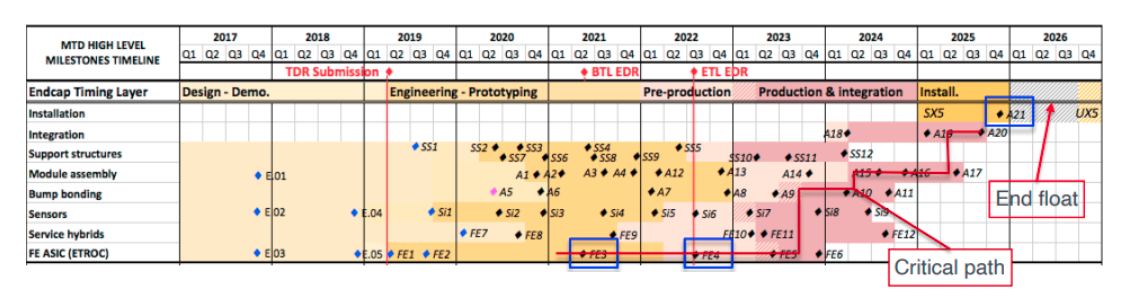
\includegraphics[width=17cm]{fig/schedule.png}
\caption{Horizonte temporal de los desarrollos del ETL en el que se incluyen los tiempos estimados para el inicio de la pre-producción y producción del ensamblado de los módulos.}
\label{fig:schedule}
\end{figure} 

\paragraph{``Commissionning'' y puesta a punto del robot de montaje\\\\}

Una de las primeras acciones a realizar consiste en la preparación del robot de montaje que será utilizado para realizar el ensamblado de los módulos. Esta tarea comenzó con anterioridad y dio lugar a un TFG y un TFM relacionado con el uso de dicho robot. Los siguientes pasos tienen que ver con la incorporación de una cámara de visión en el robot para poder realizar un alineamiento automático de los diferentes componentes del módulo; y el establecimiento de un software de control para manejar las 16 líneas de vacío necesarias en el montaje. Una vez establecidos dichos procedimiento es necesario medir la precisión espacial final que puede alcanzarse, así como los tiempos promedios necesarios para ensamblar cada módulo. Para llevar a cabo estas operaciones se dispondrá de un conjunto de piezas que emulen el montaje final de ensamblado.

\paragraph{Preparación del procedimiento de ensamblado\\\\}

Una vez los elementos técnicos del robot de montaje hayan sido probados y validados, es necesario establecer el procedimiento de montaje. Este procedimiento comienza con un sistema de registro de los componentes recibidos así como de un primer control de inspección visual para comprobar su estado. El siguiente paso consiste en la programación del robot para que sea capaz de automatizar las tareas de ensamblado, auto-calibrando su posición gracias a la visión artificial y haciendo el control efectivo de las líneas de vacío para ejercer succión sobre los componentes correspondientes. 

\paragraph{Evaluación y control de calidad de los módulos ensamblados\\\\}

Finalizado el proceso de ensamblado es preciso garantizar la calidad de los módulos producidos. Resulta por lo tanto necesario disponer de un procedimiento que garantice el correcto funcionamiento eléctrico de los módulos, así como su resistencia mecánica y térmica. Llevados a cabo los controles, los módulos producidos exitosamente han de ser registrados y almacenados para su futura instalación en el detector. 

\section{Tomografía muónica en aplicaciones industriales}

La tomografía muónica o muografía es una técnica innovadora que consiste en el uso de los muones cósmicos provenientes de las altas capas de la atmósfera para realizar inspecciones del interior de objectos de difícil acceso. Los muones interaccionan con la materia perdiendo energía y desviando su trayectoria. Cuanto más denso es el objeto, mayor es la pérdida de energía y mayor la desviación. El análisis matemático de estos observables permite la elaboración de mapas de densidad de los objetos estudiados. Existen dos tipos de tomografía muónica dependiendo del principio físico utilizado. Aquellas aplicaciones que explotan la pérdida de energía y/o atenuación de los muones son conocidas como aplicaciones de tomografía muónica de transmisión. Por el contrario, aquellas aplicaciones que utilizan la desviación angular debida al \emph{multiple scattering} sufrido por los muones, son conocidas como aplicaciones de tomografía muónica de \emph{scattering}. En este documento se hará referencia todo el rato a este último tipo de tomografía muónica. 

Esta línea de investigación persigue, de forma pionera, el estudio de esta tecnología como una técnica de ensayo no destructivo para ser utilizada en el mantenimiento preventivo de estructuras y equipamiento industrial, así como en el control de calidad de procesos productivos. Se trata por lo tanto de una línea de investigación de carácter aplicado y con una fuerte componente de transferencia tecnología. De la misma forma, se trata de una línea con un alto componente de innovación ya que la técnica es extremadamente novedosa hoy en día.   

\subsection{Experiencia previa}

\paragraph{Recostrucción de muones en el detector CMS\\\\}

El tema central de mi tesis doctoral tiene que ver con el alinemaiento de las cámaras de muones de CMS, fundamentalmente desde una perspectiva del llamado alineamiento con trazas~\cite{bib:trackbased}, pero también con contribuciones al alineamiento basado en hardware~\cite{bib:hardware1,bib:hardware2}. También fui uno de los autores de los algoritmos de reconstrucción de muones de CMS. Dichos algoritmos constituyen la base de toda la física llevada a cabo por el detector usando muones en el estado final. De la misma forma, tuve participación en los procesos de calibración de las cámaras de tubos de deriva de CMS~\cite{bib:DT1,bib:DT2,bib:DT3} y en general participé en prácticamente todas las campañas de \emph{comissionning} de los detectores de muones del experimento~\cite{bib:workflows,bib:comm,bib:mag,bib:muonreco}. En los años posteriores he participado también en otros aspectos relacionados con la detección de muones como son el trabajo en su software de DQM (\emph{Data Quality Monitoring}) y certificación, siendo el co-coordinador (L3) del grupo de \emph{DQM, validation and certification} durante los años 2017 y 2018. También he contruibido al desarrollo de algoritmos novedososo de reconstrucción como el uso de una red neuronal para estimar el momento transverso de muones de muy alto momento con alta probabilidad de haber producido \emph{showering} en el hierro del sistema de muones. Este trabajo fue recogido en un TFM en el año 2020. 


\paragraph{Tomografía muónica\\\\}

En el año 2015, mientras trabajaba como investigador postdoctoral en la ETHZ, co-fundé la compañía Muon Tomography Systems S.L., cuyo objetivo era el de desarrollar la tomografía muónica como una herramienta de ensayos no destructivos en el sector industrial. La figura~\ref{fig:tomography} (izquierda) muestra un esquema en el que dos detectores de muones son colocados antes y después de una estructura industrial. El análisis de las desviaciones angulares permite obtener información acerca de la estructura interna del objeto.

Desde el año 2015 hasta mi incorporación a la Universidad de Cantabria en el año 2017 actué como consultor científico de la compañía, contribuyendo tanto al desarrollo de sus detectores de muones como a los algoritmos de reconstrucción de imagen. En ese periodo, la empresa ganó diversas subvenciones del sector público (Gobierno del País Vasco y CDTI), así como del sector privado (Fundación Repsol). Una vez incorporado en la Universidad de Cantabria continué dicha colaboración a través de un proyecto al amparo del Artículo 83 para convenios con empresas o en el desarrollo de publicaciones conjuntas~\cite{bib:muontomography}. En el año 2018, también comencé la co-dirección de un doctorando en el marco de un doctorado industrial financiado además por el Ministerio con la subvención para la realización de doctorados industriales. Igualmente en el año 2020 dirigí un TFM con el desarrollo de un método para aplicar el principio de Maximum Likelihood para la estimación de parámetros en el contexto de la tomografía muónica.


\begin{figure}[ht]
\centering
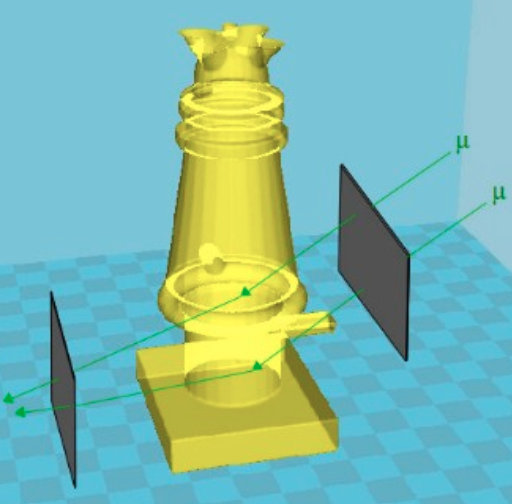
\includegraphics[height=6cm]{fig/muontomography.png}
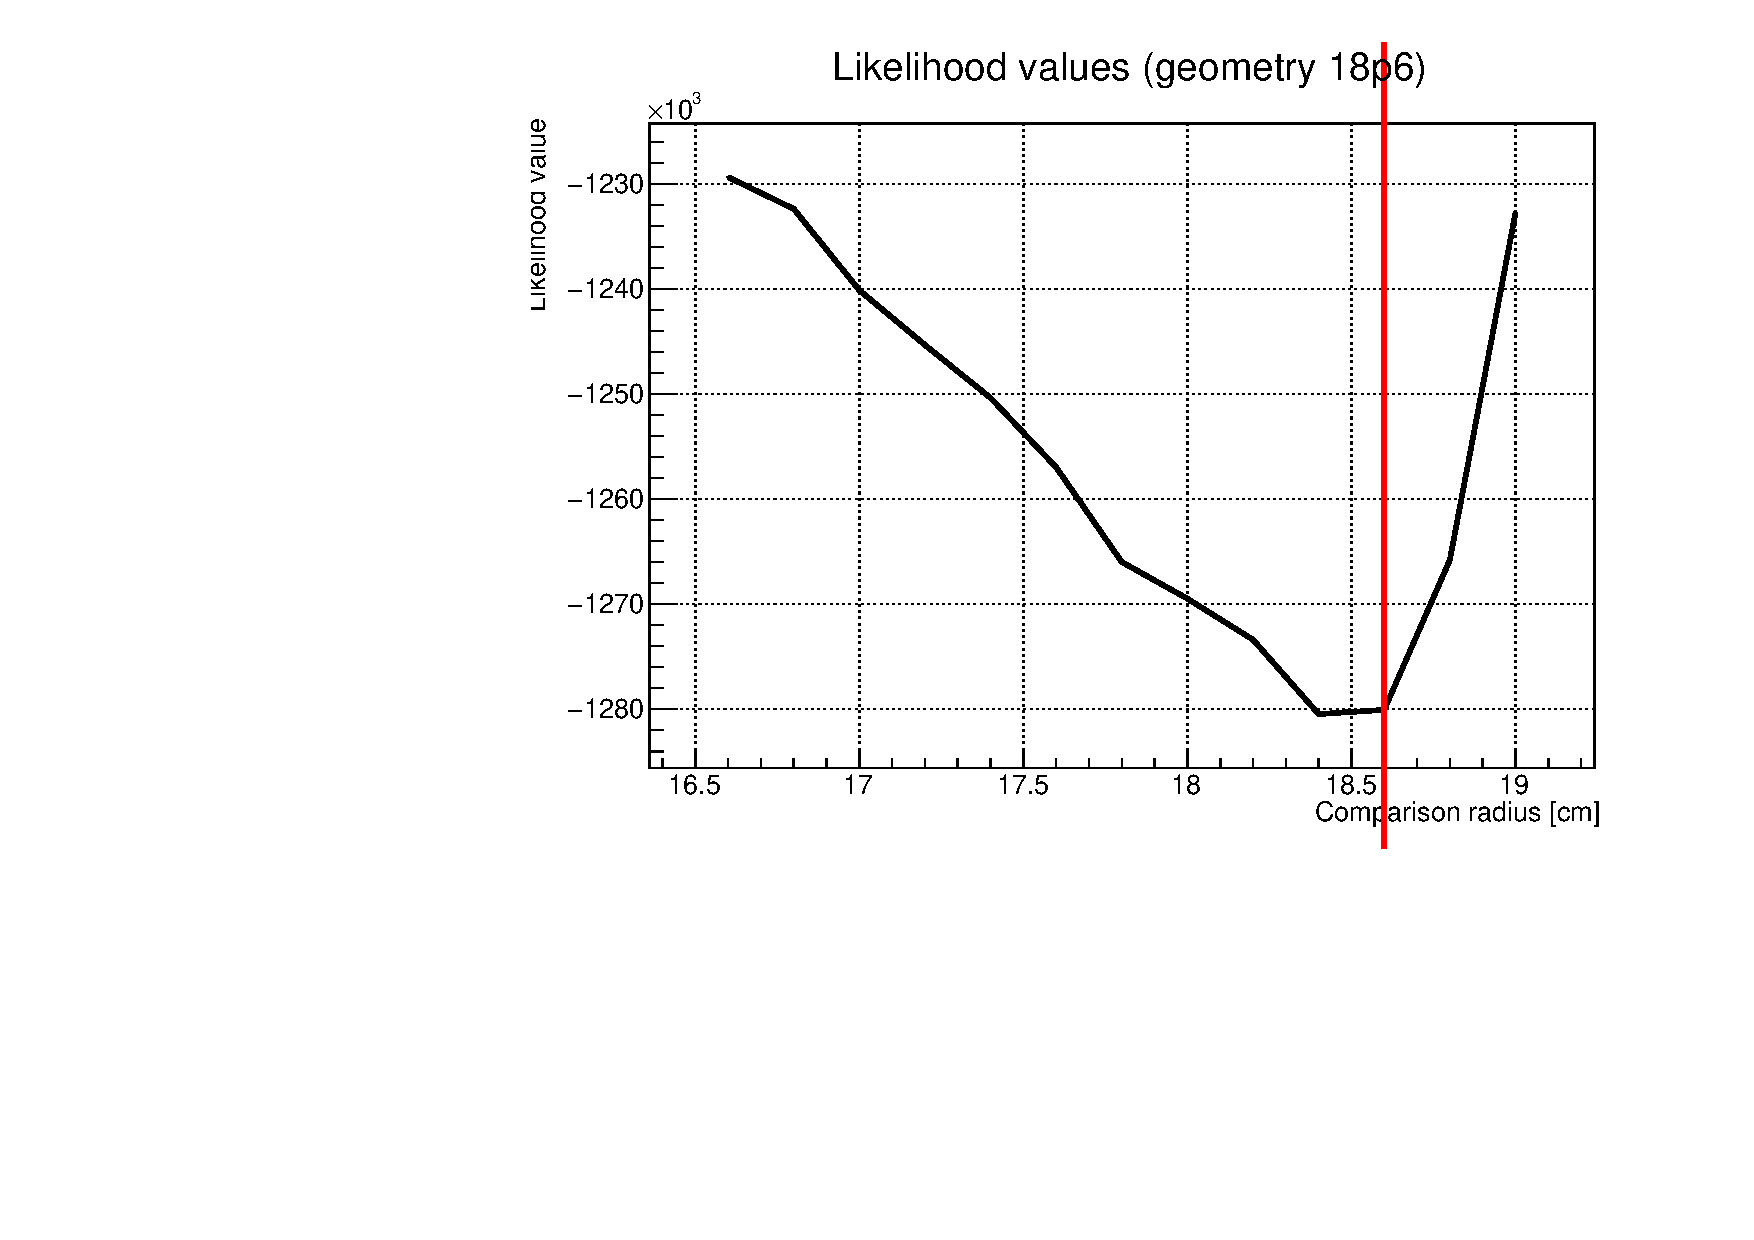
\includegraphics[height=6cm]{fig/likelihood18p6.pdf}
\caption{Esquema que muestra el modo de uso de tomografía muónica de \emph{scattering} para inferir la geometría interna de una estructura industrial (izquierda); forma del Likelihood asociado a la estimación del radio interno de una tubería en el contexto de la tomografía muónica. La línea roja muestra el valor real de dicho radio (derecha).}
\label{fig:tomography}
\end{figure} 



En el año 2018 fui invitado por la Royal Society para dar una ponencia en un congreso de Tomografía Muónica en el que participaron las 10-15 instituciones trabajando en esta técnica en el mundo. En el año 2019 fui elegido como representante español para participar en el \emph{Technical Meeting} organizado por la Agencia Internacional de la Energía Atómica (AIEA en sus siglas en inglés). Dicho encuentro propició la creación de un documento que supondrá la recomendación de la agencia a sus países miembro en lo que respecta a dicha tecnología. En la reunión fui nombrado como editor del capítulo de Tomografía Muónica en aplicaciones industriales. El documento será publicado en los próximos meses. Todos estos desarrollos han sido también presentados en varias reuniones del CPAN, así como de la Red LHC y otros workshops internacionales.   


\subsection{Desarrollo de algoritmos de reconstrucción}

Uno de los ingredientes básicos de la tomografía muónica consiste en el diseño de algoritmos que conviertan las medidas de los muones en información geométrica del sistema bajo estudio. Este problema pertenece a una categoría de problemas conocida en matemáticas como el \emph{problema inverso}, ya que tanto la información de entrada y salida del sistema, como las ecuaciones que rigen el comportamiendo del fenómeno dentro de dicho sistema son conocidas, permaneciendo como incógnitas los parámetros del sistema mismo. En el caso de la tomografía muónica este problema inverso es de naturaleza probabilística debido a la naturaleza estocástica del \emph{multiple scattering}. Existen varios algoritmos en el mercado tales como el \emph{Point of Closest Approach} (POCA)~\cite{bib:POCA} o el basado en \emph{Maximum Likelihood Estimation} (MLE)~\cite{bib:MLE} que son capaces de resolver este tipo de problemas aunque con grandes limitaciones en cuanto a la resolución espacial final obtenida. En esta línea de inestigación se persigue el desarrollo de algoritmos más precisos.  

\paragraph{Algoritmos de baja dimensión paramétrica\\\\}

Una de las razones para iniciar el uso de la tomografía muónica en aplicaciones industriales tiene que ver con la naturaleza de sus problemas. Al contrario que en otros sectores, normalmente en las aplicaciones industriales se dispone de un conocimiento muy preciso de la geometría nominal de las estructuras estudiadas. En la mayor parte de los casos se persigue estimar el nivel de desgaste o la aparición de defectos que pueden verse como pequeñas variaciones geométricas  sobre una geometría nominal bien conocida. Este hecho permite reducir dramáticamente la complejidad del problema inverso ya que con frecuencia puede reducirse la inferencia a unos pocos parámetros. Un ejemplo paradigmático puede encontrarse en una de las aplicaciones tratadas en los últimos años: la medida del desgaste de tuberías transportadoras de gas. En este problema, y a primer orden, existe un único parámetro de interés: el radio interno de la tubería que determina su grosor y por tanto el nivel de desgaste. Esta reducción en la dimensión parámetrica hace que estos problemas sean idóneos para tratamientos como el que ya se realizó basado en \emph{Maximum Likelihoods} (ver Fig.~\ref{fig:tomography}, derecha), o de forma aún más interesante, para el uso de redes neuronales profundas que funcionen en modo de regresión a los parámetros de interés. En esta sublínea de trabajo se buscará el desarrollo de este tipo de algoritmos prestando atención a sus posibilidades de entrenamiento tanto con datos reales como con datos simulados.

\paragraph{``Machine-learning Optimized Design of Experiments''\\\\}

En el año 2021 me convertí formalmente en miembro de la colaboración MODE\footnote{https://mode-collaboration.github.io/} (\emph{Machine-learning Optimized Design of Experiments}) cuyo objetivo principal es fomentar y avanzar en la producción de algoritmos de \emph{Machine Learning} que faciliten la optimización y el diseño de experimentos. La colaboración MODE aglutina a una veintena de expertos en Estadística, Machine Learning y Física Experimental de Altas Energías. Los objetivos de la colaboración MODE son muy generales, ya que su diseño de algoritmos tiene la vocación de convertirse en un estándar para el diseño de experimentos, no exclusivamente de Física de Partículas. Por otro lado, con objeto de avanzar en este propósito, la colaboración ha elegido un conjunto de casos de uso, entre los cuáles el más importante y avanzado es el de la tomografía muónica. 

Durante los próximos años, un conjunto de 5 miembros de la colaboración, estamos inmersos en la escritura de un software basado en el principio de \emph{Differential Programming}~\cite{bib:differentialprogramming}, que hace uso de algoritmos secuenciales con capacidad para ser diferenciados y usados en procesos de minimización, para resolver el problema inverso asociado a la tomografía muónica de scattering. 

Cabe destacar que si bien mi actividad actual en este grupo queda enmarcada en el contexto de la tomografía muónica, mi interés va más allá y en el futuro se perseguirán contribuciones más generales en relación con el concepto de diseño de experimentos optimizado con técnicas de Machine-learning.

\subsection{Desarrollo de simulaciones basadas en redes adversarias}

Muchos de los algoritmos de tomografía muónica mencionadados anteriormente requieren una gran cantidad de simulación para ser entrenados. Tradicionalmente la simulación del paso de las partículas a través de la materia suele hacerse con el paquete GEANT4, que a pesar de estar altamente optimizado, presenta una gran complejidad computacional debido al nivel de detalle con el que produce las simulaciones. Con objeto de reducir estos tiempos, se plantea una línea de investigación que persiga la generación de simulaciones realistas de escenarios de tomografía muónica utilizando \emph{Redes Neuronales Adversarias} (GAN)~\cite{gan}. Estas redes funcionan con un principio de competición entre una red generadora que intenta crear simulaciones realistas a partir de entradas aleatorias, y una red discriminadora que persigue diferenciar si la información ofrecida como entrada es real o ha sido generada por la red. En el proceso de minimización conjunto es posible conseguir un generador con capacidad de producir simulaciones muy realistas.

\subsection{Medida del momento: tomografía muónica y LGADs}

Dentro del IFCA y en colaboración con el Centro Nacional de Microelectrónica (CNM) y el Instituto Tecnológico de Aragón (ITAINNOVA), estoy liderando una iniciativa para mejorar los dispositivos de tomografía muónica con el uso de LGADs para medir el tiempo de paso de los muones por los detectores. A través de la diferencia temporal y del espacio recorrido es posible estimar la velocidad del muon y con ello su momento. 

Es preciso destacar que los algoritmos de tomografía muónica sufren una grave pérdida de resolución debida a que la desviación angular de los muones no solo depende de las propiedades del material sino también de su momento. Tradicionalmente los experimentos de física de partículas estiman el momento a través de la medida de la curvatura de los muones en campos magnéticos intensos, sin embargo, este tipo de tecnología no resulta rentable para aplicaciones industriales. Por lo tanto, hasta la fecha todos los intentos de tomografía muónica han promediado el momento de los muones con la consecuente pérdida de resolución. Un sistema como el propuesto aquí es por lo tanto único y revolucionario dentro del campo. 

Esta línea de investigación será desarrollada en el contexto del programa de Prueba de Concepto asociado al plan estatal. El proyecto ha sido concedido y se espera que entre en vigor en los próximos meses. El proyecto tiene como objetivo hacer una prueba de concepto con sensores LGAD y su correspondiente electrónica, capaces de proporcionar una resolución temporal de 50~ps, y con una superficie de detección de pocos centímetros. Dentro del proyecto se estudiarán también algoritmos de reconstrucción que sean capaces de explotar la información del momento, así como la escalabilidad del sistema para superficies de detección más extensas.


\section{Futuros aceleradores}

En el año 2019 tuvo lugar en Granada el \emph{Open Symposium - Update of the European Strategy for Particle Physics}. Este evento, en el que participé, junto con una parte muy significativa de la comunidad europea de física de partículas, sirvió para discutir los pilares básicos de la estrategia europea de física de partículas para los años venideros. En el año 2020, el \emph{European Strategy for Particle Physics Group} elaboró un documento~\cite{future} recogiendo las conclusiones de este proceso, estableciendo las líneas estratégicas principales de la comunidad de física de partículas europea. 

Este documento reconoce como máxima prioridad la construcción de un colisionador electrón-positrón que suponga una factoría de bosones de Higgs. En el largo plazo, se reconoce la ambición de construir un colisionador protón-protón con la máxima energía alcanzable posible. Para perseguir estos objetivos, la comunidad de física de partículas debe comenzar sus esfuerzos de investigación y desarrollo en tecnologías de aceleración avanzadas y particularmente en el desarrollo de imanes de superconductor de alto campo, incluyendo superconductores de alta temperatura. La comunidad debe investigar la viabilidad técnica y financiera de un futuro colisionador de hadrones en el CERN con una energía del centro de masas de al menos 100~TeV, que tenga a un acelerador electrón-positrón para estudiar las propiedades del bosón de Higgs como etapa previa. A la vez, la estrategia considera compatibles estos esfuerzos con la construcción del \emph{International Linear Collider (ILC)} en Japón, en el que la comunidad europea desería colaborar. En segundo lugar, la estrategia subraya la importancia de intensificar y financiar adecuadamente la investigación en nuevas tecnologías de aceleración, especialmente imanes de alto campo, superconductores de alta temperatura, aceleración con \emph{plasma wakefield} y otras estructuras de aceleración de alto gradiente, entre otras. 

En este contexto, se propone esta línea de investigación a largo plazo, que tendrá como primer objetivo el posicionamiento científico de cara a los nuevos desarrollos y aceleradores, en congruencia con los intereses de la comunidad de física de partículas española y en última instancia con las líneas generales de la estrategia europea. Este posicionamiento desembocará en el futuro en la participación en los próximos esfuerzos de la comunidad.





